\section{\Large ATTITUDE DETERMINATION}
\subsection{Attitude Control Error}
In operation, NISAR will point its antenna towards Earth such that the principal x-axis facing the negative radial direction and the principal y-axis is pointing in the negative normal direction. The angular velocity about the principal y-axis is the negative of mean motion.
\begin{align*}
    \Vec{P}_{desired} &= 
    \begin{bmatrix}
    -1 & 0 & 0 \\
    0 & 0 & -1 \\
    0 & -1 & 0
    \end{bmatrix}
    \Vec{P}_{RTN}
\end{align*}
We first simulate attitude without disturbance torques, calculating error as the rotation between target and actual attitude. Figures \ref{fig:Images/ps6_problem2_principal}, \ref{fig:Images/ps6_problem2_target}, \ref{fig:Images/ps6_problem2_error} demonstrate that the error is approximately zero.

\begin{figure}[H]
\centering
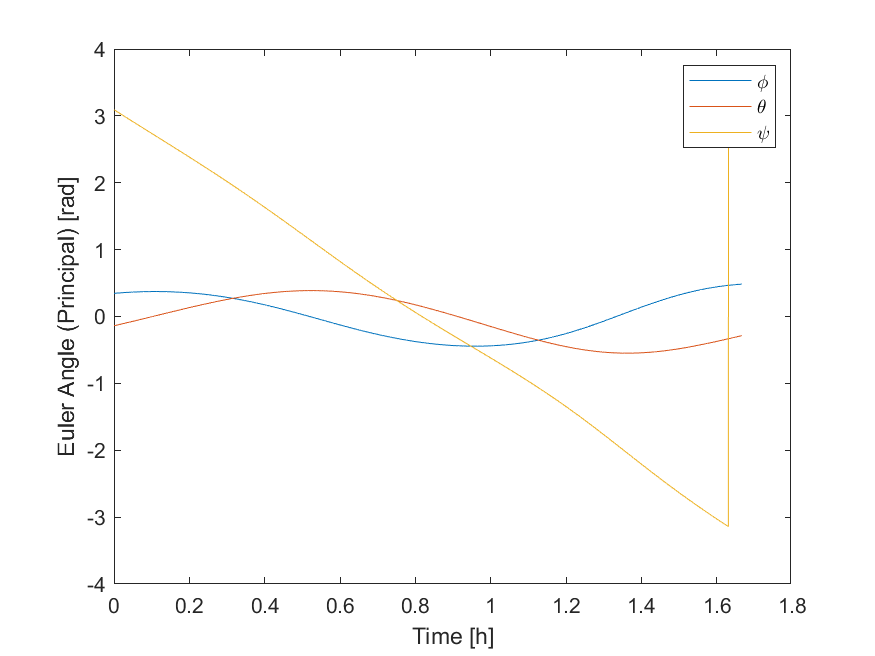
\includegraphics[scale=0.6]{Images/ps6_problem2_principal.png}
\caption{Actual attitude relative to inertial frame, without perturbations}
\label{fig:Images/ps6_problem2_principal}
\end{figure}

\begin{figure}[H]
\centering
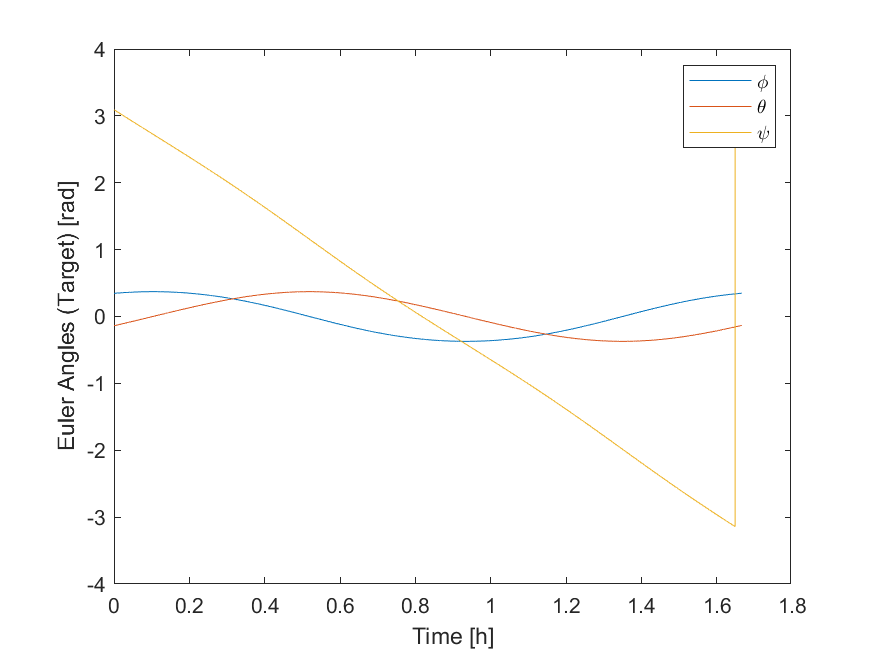
\includegraphics[scale=0.6]{Images/ps6_problem2_target.png}
\caption{Target attitude relative to inertial frame, without perturbations}
\label{fig:Images/ps6_problem2_target}
\end{figure}

\begin{figure}[H]
\centering
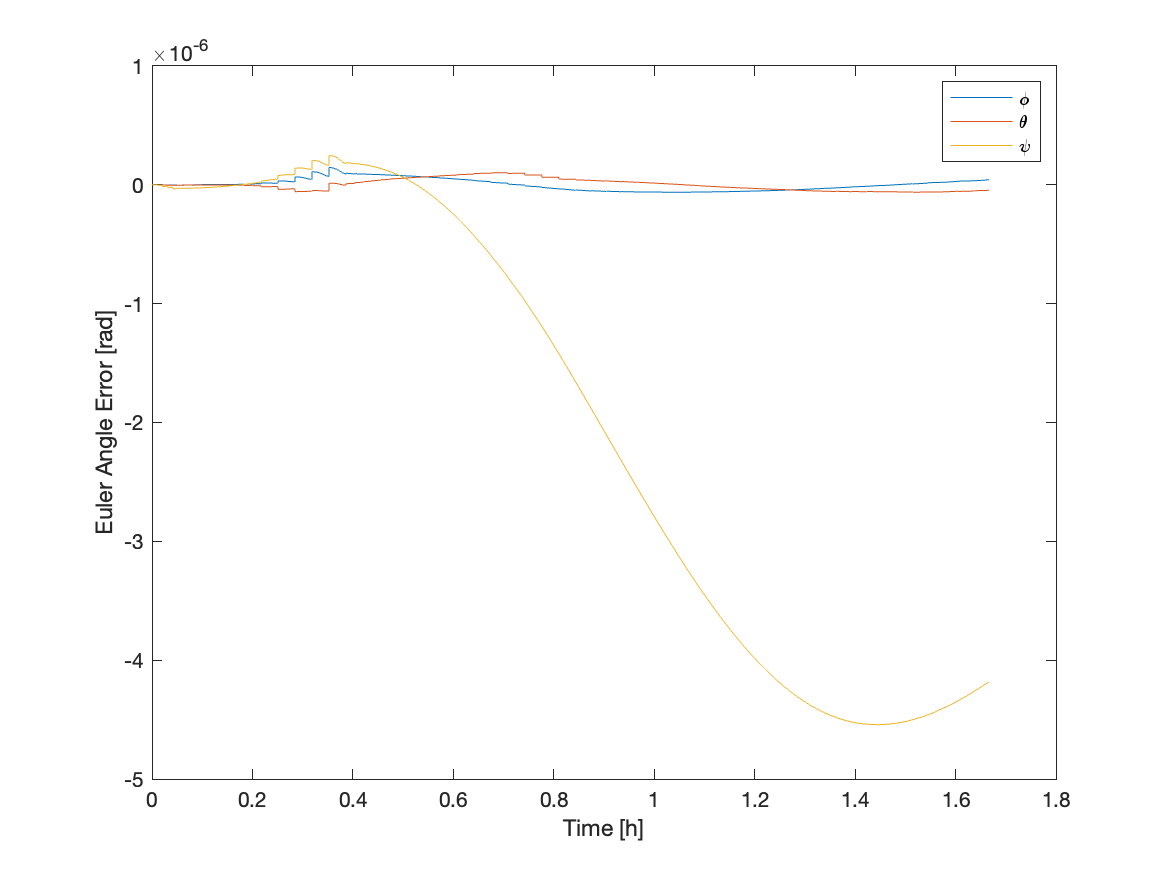
\includegraphics[scale=0.6]{Images/ps6_problem2_error.png}
\caption{Error between target and actual attitude, without perturbations}
\label{fig:Images/ps6_problem2_error}
\end{figure}

For computing errors, we multiply the DCM representing the rotation from the inertial frame to our actual attitude with the inverse of the DCM representing the rotation from the inertial frame to the target attitude. We observe that there is a very small error (approximately $10^{-7}$ to $10^{-6}$) in our result in Figure \ref{fig:Images/ps6_problem2_error}. This is most likely arising from our use of numerical integration.

\subsection{Attitude Control Error, with Perturbation}
With perturbations, we observe a small but noticeable change to actual attitude in Figure \ref{fig:Images/ps6_problem3_principal}.

\begin{figure}[H]
\centering
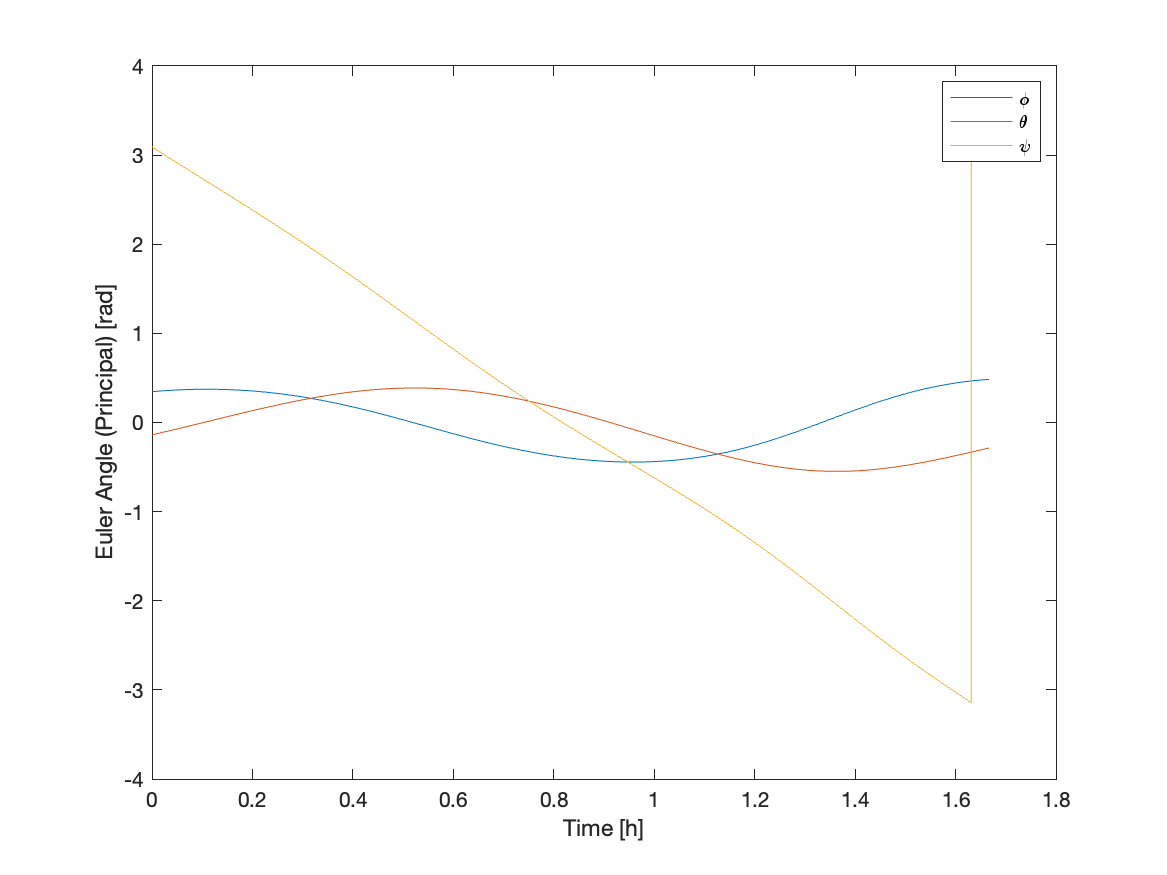
\includegraphics[scale=0.6]{Images/ps6_problem3_principal.png}
\caption{Actual attitude relative to inertial frame, with perturbations}
\label{fig:Images/ps6_problem3_principal}
\end{figure}

\begin{figure}[H]
\centering
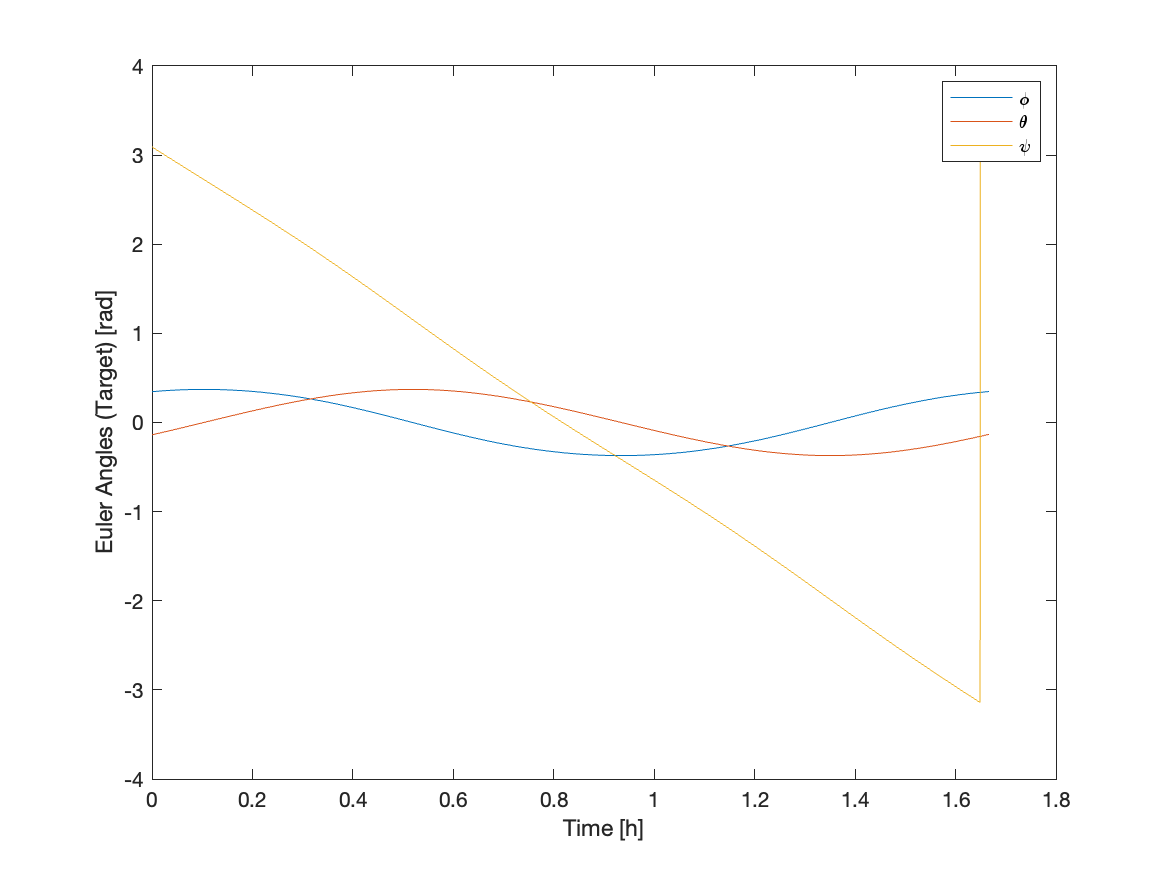
\includegraphics[scale=0.6]{Images/ps6_problem3_target.png}
\caption{Target attitude relative to inertial frame, with perturbations}
\label{fig:Images/ps6_problem3_target}
\end{figure}

A much larger error appears in Figure \ref{fig:Images/ps6_problem3_error}. When compared with the disturbance-free error in Figure \ref{fig:Images/ps6_problem2_error} (which is approximately zero), we can interpret the attitude control error as the amount which the disturbance torques rotate our satellite during the simulation period, which in this case is one orbital period.

\begin{figure}[H]
\centering
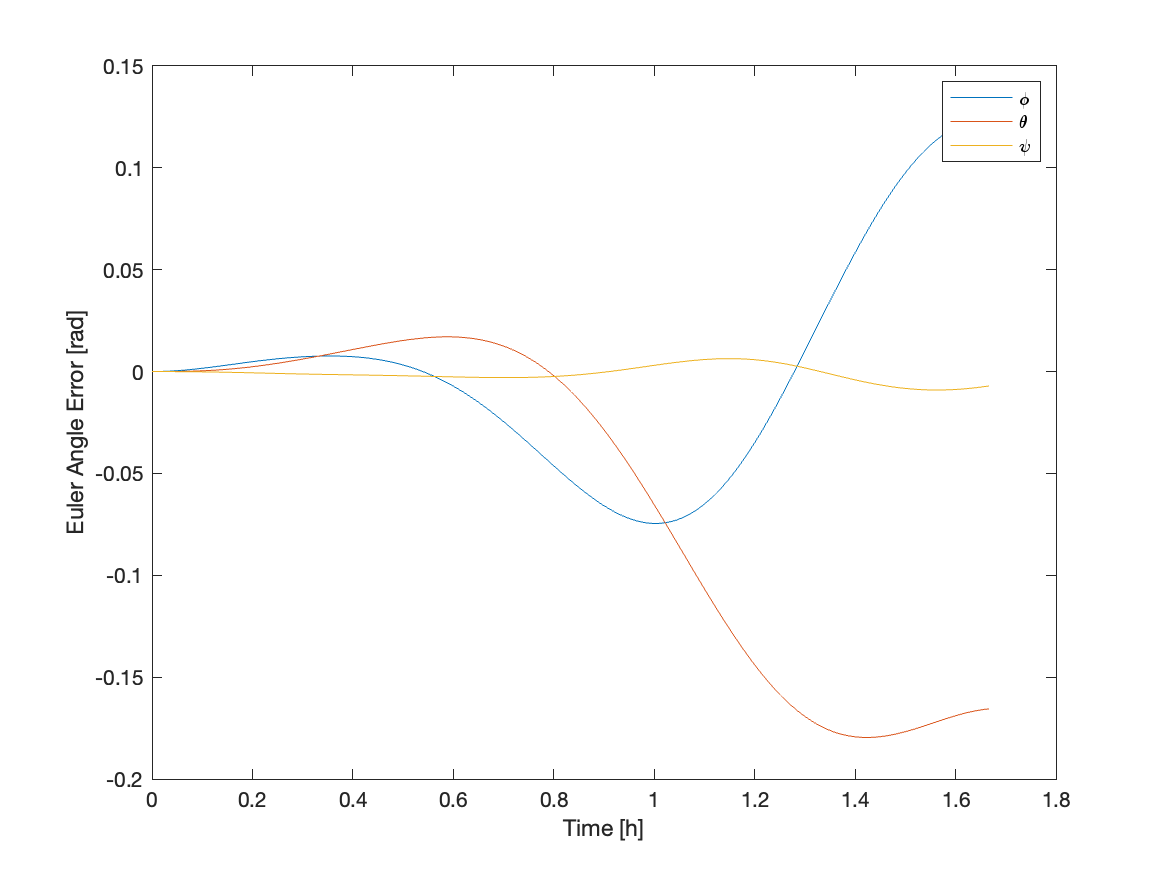
\includegraphics[scale=0.6]{Images/ps6_problem3_error.png}
\caption{Error between target and actual attitude, with perturbations}
\label{fig:Images/ps6_problem3_error}
\end{figure}

\subsection{Attitude Determination Subsystem}
We create a Simulink model using the same functions and variables previously modeled in MATLAB and shown in this paper, shown in Figure \ref{fig:Images/ps6_problem4}. Notably, we have a simulation subsystem which is responsible for simulating the dynamics, kinematics, and disturbances of the system, which we have modeled in previous sections. We now add an attitude determination subsystem for this step. Since we choose to model noise-free measurements for now, we directly generate measurements from the true state without injecting noise.

We initially model our attitude determination subsystem using ``dummy'' sensors and measurements. Each of the algorithms is fed randomly generated unit vectors as a noise-free measurement. These unit vectors represent fixed directions in the celestial sphere such that an orientation can be computed when a sufficient number of vectors is available. This represents the functionality of a star tracker sensor, which is able to determine the orientation of the satellite's axes relative to an inertial reference using unit vector directions of known stars. We do not yet model the inner workings of a star tracker, such as the identification and computation of star positions.

In our test implementation, we generate five such random unit vectors. These unit vectors are both our ground truth (analogous to known directions from a star catalog) and our measurement signal, since we do not inject any noise at this step. Thus, we expect to obtain an exact solution from each attitude determination algorithm in the absence of such noise.

\begin{figure}[H]
\centering
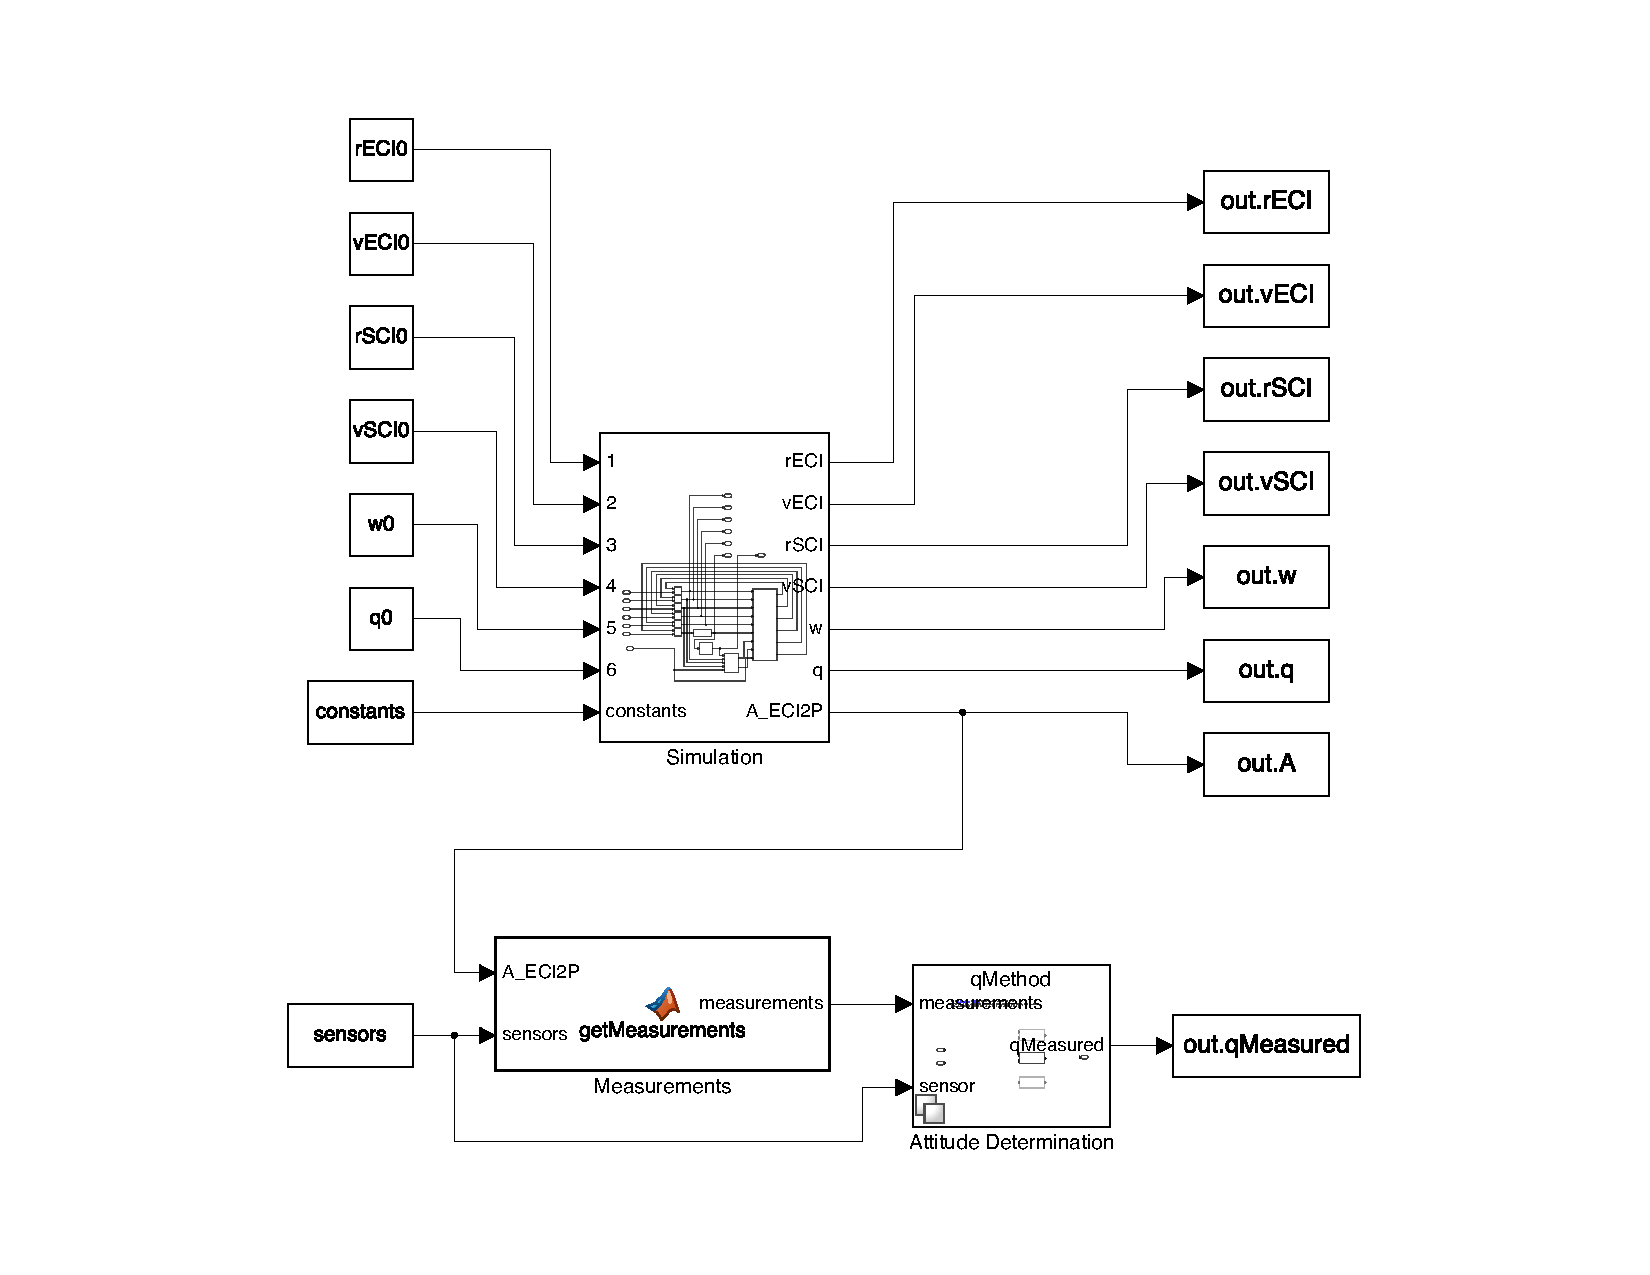
\includegraphics[scale=0.55]{Images/ps6_problem4.pdf}
\caption{Simulink model for NISAR spacecraft}
\label{fig:Images/ps6_problem4}
\end{figure}

Additionally, we can compute the attitude by integration of our angular velocity, equivalent to using a rate gyro sensor that measures angular rate. We can simply use the same kinematics equations used to propagate our attitude to model the evolution of our attitude for the rate gyro. In simulation and without noise, we also expect an exact solution from this technique.

\subsection{Deterministic Attitude Determination Algorithm}
For measurements $\Vec{M}$ and ground truth $\Vec{V}$, we can use deterministic attitude determination to find the attitude by taking the pseudoinverse.
\begin{align*}
    \Vec{M} &= 
    \begin{bmatrix}
        \vdots & \vdots & \vdots\\
        \Vec{m}_{1} & \Vec{m}_{2} & \Vec{m}_{3}\\
        \vdots & \vdots & \vdots
    \end{bmatrix} =
    \Vec{A} \begin{bmatrix}
        \vdots & \vdots & \vdots\\
        \Vec{v}_{1} & \Vec{v}_{2} & \Vec{v}_{3}\\
        \vdots & \vdots & \vdots
    \end{bmatrix} =
    \Vec{A} \Vec{V} \\
    \Vec{A} &= \Vec{M} \Vec{V}^{-1}
\end{align*}
The implementation of the deterministic attitude determination method above assumes that we have three or more measurements. However, if there are only two measurements, a third measurement can be ``created'' using the cross product. This technique creates measurements and corresponding ground truth vectors $p$, $q$, and $r$ as shown below.
\begin{align*}
    \Tilde{\Vec{{m}}}_1 = \frac{\Vec{m}_1 + \Vec{m}_2}{2} \;\;\;
    \Tilde{\Vec{{m}}}_2 = \frac{\Vec{m}_1 - \Vec{m}_2}{2} \;\;\;
    \Tilde{\Vec{{v}}}_1 = \frac{\Vec{v}_1 + \Vec{v}_2}{2} \;\;\;
    \Tilde{\Vec{{v}}}_2 = \frac{\Vec{v}_1 - \Vec{v}_2}{2} \\
    \Vec{p}_m = \Tilde{\Vec{{m}}}_1; \;\;\;
    \Vec{{q}}_m = \frac{\Tilde{\Vec{{m}}}_1 \times \Tilde{\Vec{{m}}}_2}{||\Tilde{\Vec{{m}}}_1 \times \Tilde{\Vec{{m}}}_2||} \;\;\;
    \Vec{{r}}_m = \Vec{p}_m \times \Vec{v}_m \\
    \Vec{p}_v = \Tilde{\Vec{{v}}}_1; \;\;\;
    \Vec{{q}}_v = \frac{\Tilde{\Vec{{v}}}_1 \times \Tilde{\Vec{{v}}}_2}{||\Tilde{\Vec{{v}}}_1 \times \Tilde{\Vec{{v}}}_2||} \;\;\;
    \Vec{{r}}_v = \Vec{p}_v \times \Vec{v}_v \\
\end{align*}

\subsection{Statistical Attitude Determination Algorithm (q-Method)}
Given measurements $\Vec{M}$, ground truth $\Vec{V}$, and sensor weights $\Vec{W}$, we can use statistical attitude determination (aka the q-method). This method ultimately finds the quaternions using the eigenvalue/eigenvector below, where the eigenvector associated with the largest eigenvalue is the quaternion vector.
\begin{align*}
    \Vec{K} \Vec{q} = \lambda \Vec{q}
\end{align*}
In the eigenvalue decomposition above, $\Vec{K}$ can be found with the following relation.
\begin{align*}
    \Vec{w}_i = \sqrt{w_1} \Vec{m}_1 \;\;\;
    \Vec{u}_i = \sqrt{w_1} \Vec{v}_1 \\
    \Vec{W} = 
    \begin{bmatrix}
        \Vec{w}_1 & \Vec{w}_2 & ... & \Vec{w}_n
    \end{bmatrix} \;\;\;
    \Vec{U} = 
    \begin{bmatrix}
        \Vec{u}_1 & \Vec{u}_2 & ... & \Vec{u}_n
    \end{bmatrix} \\
    \Vec{B} = \Vec{W} \Vec{U}^T \;\;\;
    \Vec{S} = \Vec{B} + \Vec{B}^T \;\;\;
    \sigma = trace (\Vec{B}) \\
    Z = 
    \begin{bmatrix}
        B_{23} - B_{32} & B_{31} - B_{13} & B_{12} - B_{21}
    \end{bmatrix} ^T \\
    K = 
    \begin{bmatrix}
        \Vec{S} - \sigma \Vec{I} & \Vec{Z} \\
        \Vec{Z}^T & \sigma
    \end{bmatrix}
\end{align*}

\subsection{Kinematic Attitude Determination Algorithm}
We can reconstruct our attitude using the kinematic equations used to model our attitude motion in the ground truth simulation, instead simulated as part of the spacecraft's onboard computer. We simply duplicate our previously-implemented kinematic equations and pass in the angular velocity to reconstruct attitude evolution for this technique.

The methods for attitude determination are implemented in MATLAB code included in the appendix. We include implementations for deterministic attitude determination both for two measurements and for three or more measurements.

\subsection{Attitude Estimation, without Sensor Errors}
Figures \ref{fig:Images/ps6_problem6_actual}, \ref{fig:Images/ps6_problem6_DAD}, \ref{fig:Images/ps6_problem6_DADFict}, and \ref{fig:Images/ps6_problem6_qMethod} depict the attitude determination using the different methods discussed earlier. All are identical, which is expected, since each algorithm is given perfect measurements free of noise. Error for each is on the order of $10^{-16}$, which is purely numerical.

\begin{figure}[H]
\centering
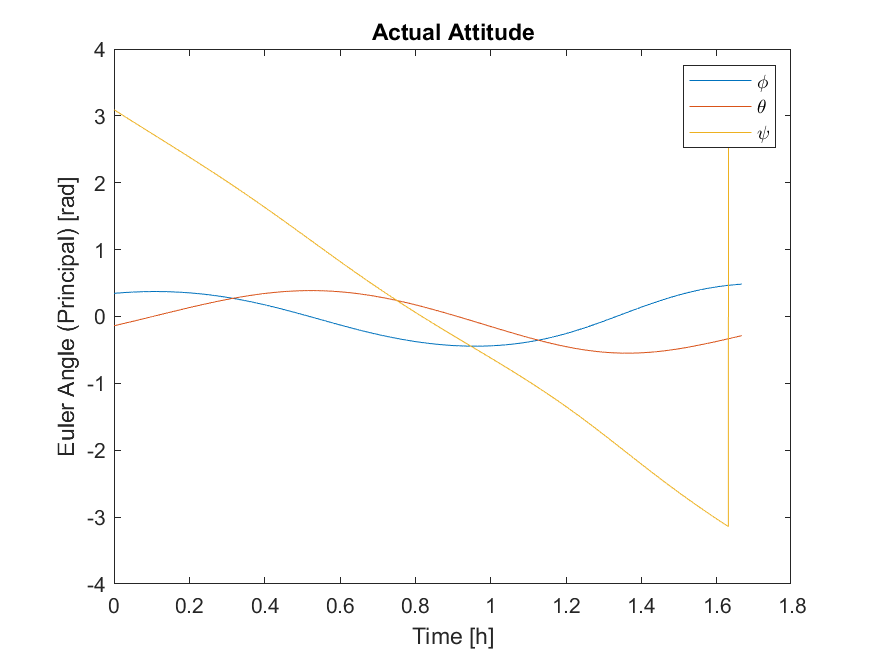
\includegraphics[scale=0.8]{Images/ps6_problem6_actual.png}
\caption{True satellite attitude relative to inertial frame}
\label{fig:Images/ps6_problem6_actual}
\end{figure}

\begin{figure}[H]
\centering
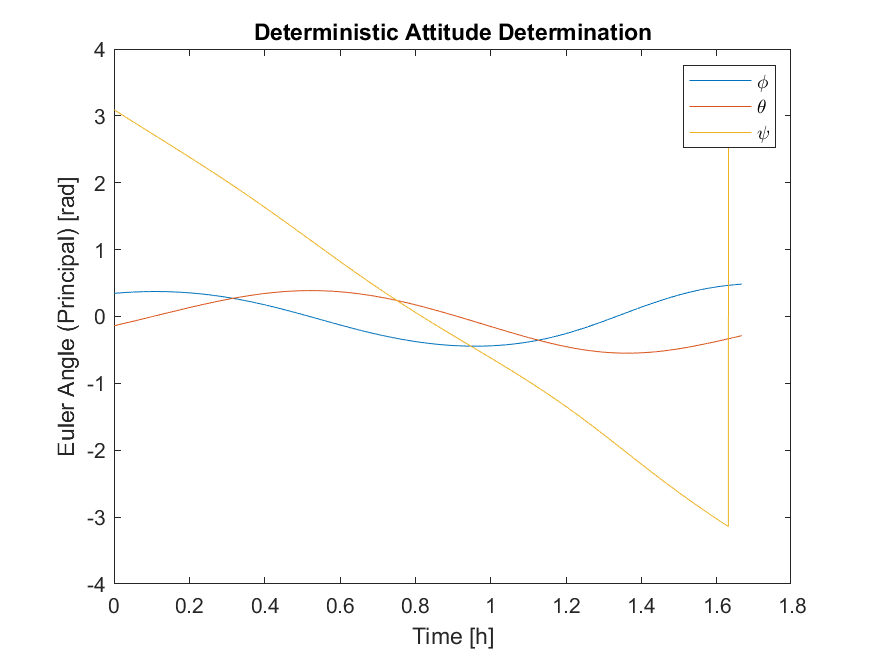
\includegraphics[scale=0.8]{Images/ps6_problem6_DAD.png}
\caption{Deterministic attitude determination}
\label{fig:Images/ps6_problem6_DAD}
\end{figure}

\begin{figure}[H]
\centering
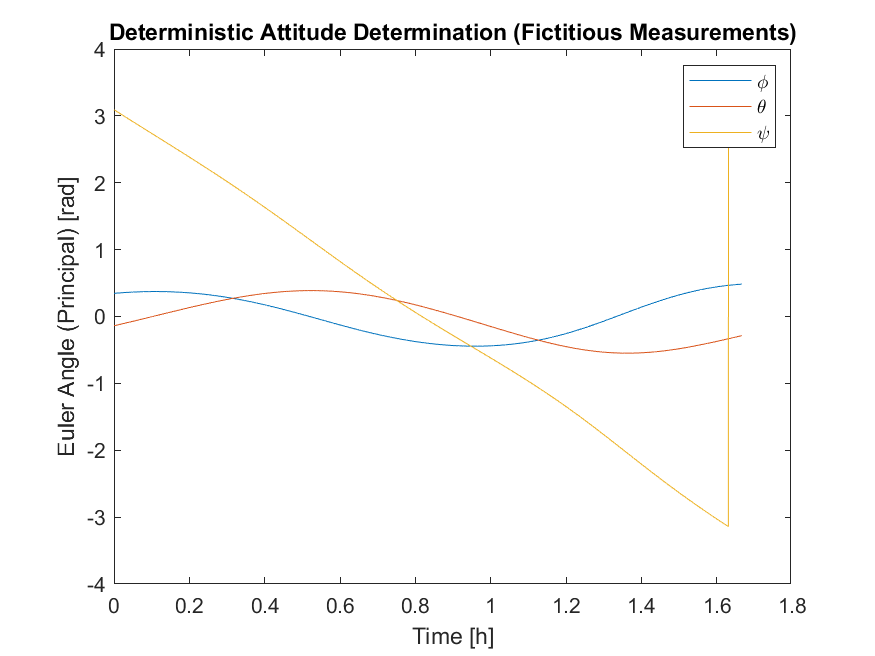
\includegraphics[scale=0.8]{Images/ps6_problem6_DADFict.png}
\caption{Deterministic attitude determination with fictitious measurements}
\label{fig:Images/ps6_problem6_DADFict}
\end{figure}

\begin{figure}[H]
\centering
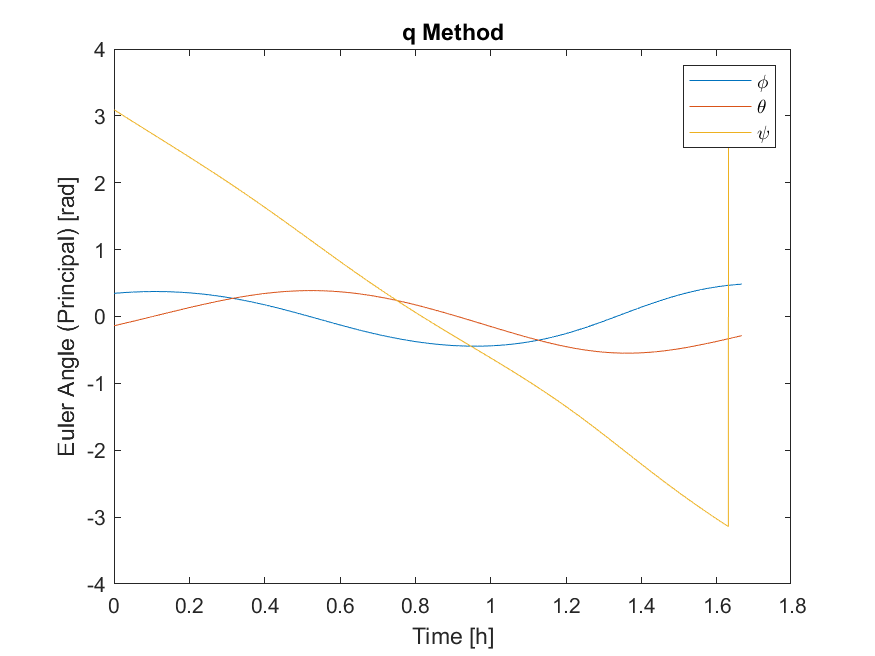
\includegraphics[scale=0.8]{Images/ps6_problem6_qMethod.png}
\caption{q-method}
\label{fig:Images/ps6_problem6_qMethod}
\end{figure}

\begin{figure}[H]
\centering
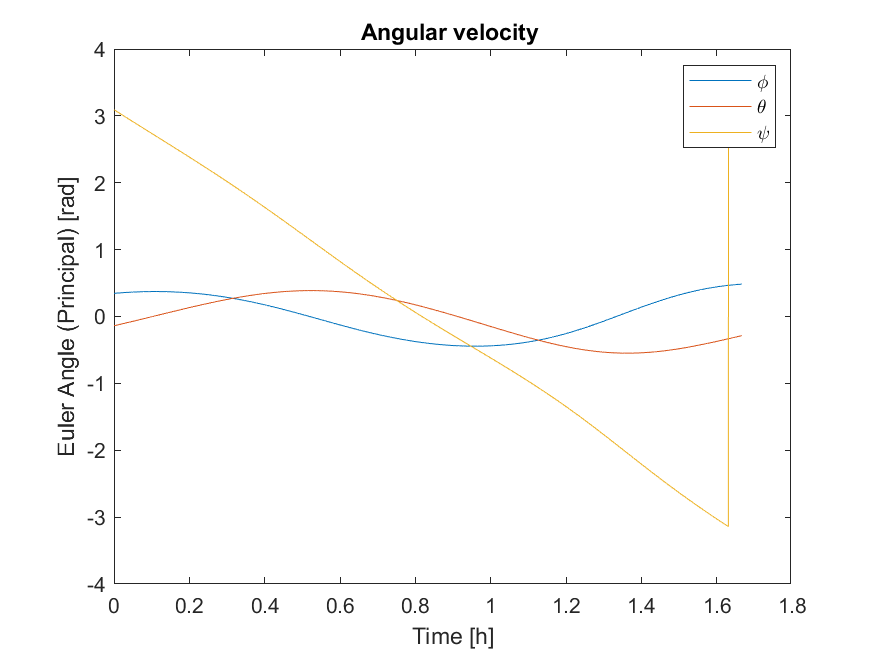
\includegraphics[scale=0.8]{Images/ps6_problem6_kins.png}
\caption{Attitude reconstruction using kinematic equations}
\label{fig:Images/ps6_problem6_kins}
\end{figure}

\subsection{Sensor Specifications}
As the specific data regarding for NISAR ADCS sensors are not widely available, much of the sensor error and bias information was extrapolated from data from Wertz and lecture materials, as well as manufacturers of sensors for similar satellites. The table below includes the general sensor information used in this analysis.

\begin{table}[H]
\caption{Sensor performance specifications}
\centering
\begin{tabular}{|l|l|l|}
\hline
\textbf{Sensor} & \textbf{Sensor Error} & \textbf{Sensor Bias} \\ \hline
Sun Sensor \cite{Wertz} & 0.5\degree & 0\degree \\ \hline
Star Tracker \cite{Wertz} & 0.01\degree & 0\degree \\ \hline
Gyroscope \cite{CVGGyro} & 0.001\degree / s & 5E-5\degree/s \\ \hline
\end{tabular}
\end{table}

\subsection{Attitude Estimation, with Sensor Errors}
The estimation errors for the deterministic method, q-method, and kinematics-based method are plotted below. As expected, the q-method has a significantly lower error than the deterministic method. Additionally, since the gyroscopes were modeled to have a slight bias, the Euler angles slowly drift away from expected values.

\begin{figure}[H]
\centering
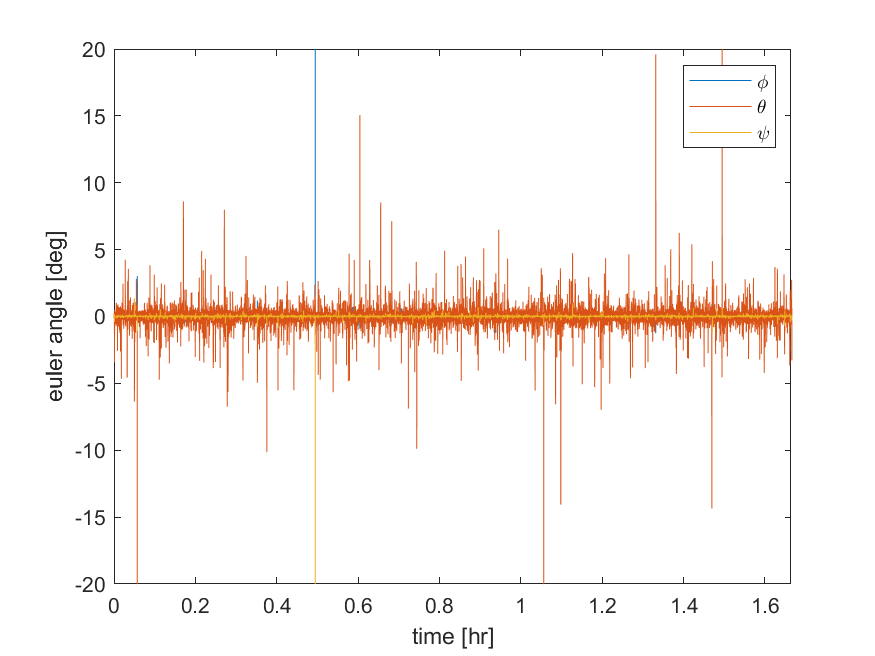
\includegraphics[scale=0.6]{Images/ps7_problem2_DADFict.png}
\caption{Attitude error using deterministic attitude determination}
\label{fig:ps7_problem2_DADFict}
\end{figure}

\begin{figure}[H]
\centering
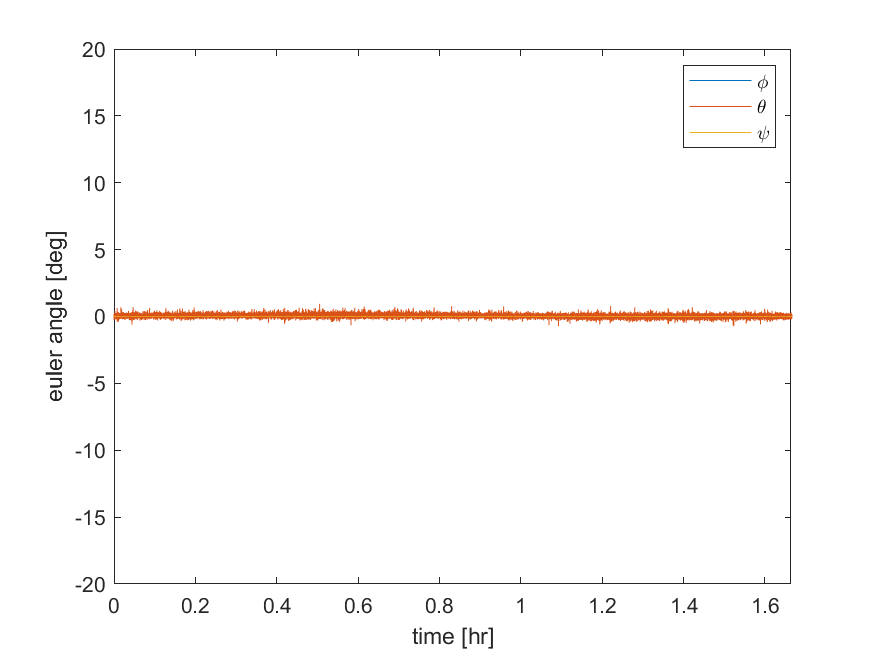
\includegraphics[scale=0.6]{Images/ps7_problem2_qMethod.png}
\caption{Attitude error using q-method}
\label{fig:ps7_problem2_qMethod}
\end{figure}

\begin{figure}[H]
\centering
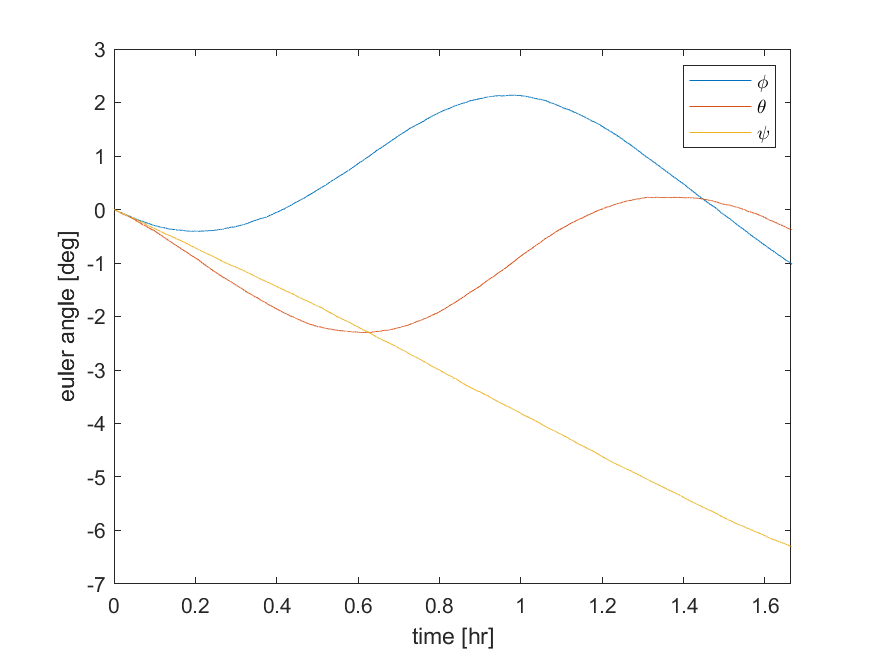
\includegraphics[scale=0.6]{Images/ps7_problem2_kin.png}
\caption{Attitude error using kinematic attitude determination}
\label{fig:ps7_problem2_kin}
\end{figure}

\subsection{Small Angle Errors}
For this analysis, we choose to use q-method, as it produced the smallest errors in the previous section. In order to estimate the size of the errors, we compare the exact error DCM to the small angle approximation DCM based on the corresponding Euler angles, shown below.
\begin{align*}
    A_{\text{small angle}} &= 
    \begin{bmatrix}
        1 & \phi & -\psi \\
        -\phi & 1 & \theta \\
        \psi & -\theta & 1
    \end{bmatrix}
\end{align*}
The Frobenius norm is then calculated from the difference in the error DCM and small angle DCM to see how applicable small angle assumptions are for the error. Based on Figure \ref{fig:ps7_problem3}, the magnitudes of the Frobenius norm reflect that the overall errors were relatively small for the q-method, implying only a very small angular difference.

\begin{figure}[H]
\centering
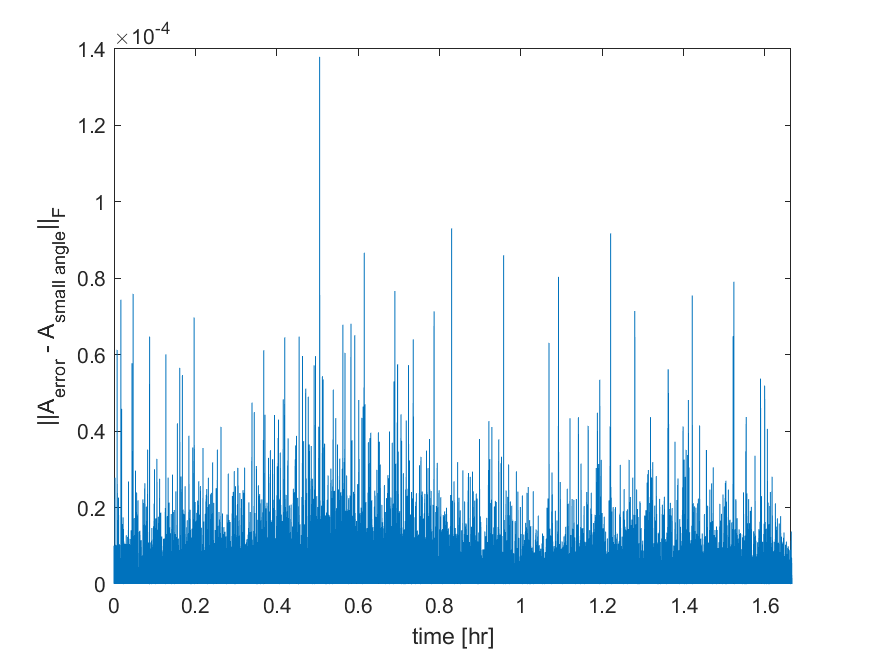
\includegraphics[scale=0.6]{Images/ps7_problem3.png}
\caption{Frobenius norm of error estimate versus small angle approximation}
\label{fig:ps7_problem3}
\end{figure}

\subsection{Sensor Models}
There are three major types of sensors used in this analysis: sun sensors, star sensors, and gyroscopes. The following section discusses the basics of each sensor's function and modeling.

Sun sensors utilize a photoelectric effect to produce an electric current based on the Sun's emitted electromagnetic radiation. For a single sensor, the current is based on sensitive surface $S$, optical properties $\alpha$, and angle of incidence $\theta$.
\begin{align*}
    I = \alpha S \cos(\theta)
\end{align*}
Due to the nonlinearity of this relationship, sun sensors operate within a limited field of view where the relationship between the angle of incidence and current draw is approximately linear.

However, because NISAR operates in a sun-synchronous orbit, the sun sensor model we used did not factor in the sensor's field of view, as a well-placed sensor with a wide enough FOV will always have the sun in frame. Our sun sensor model outputs the direction of the Sun from the simulation and adds Gaussian noise.

Star trackers are more complicated. These sensors are similar to cameras that capture star positions and compare them to an existing star catalog, which can be used to determine the satellite's attitude. These trackers are often designed to have a much narrower field of view to maximize the pixel pitch. Star trackers use algorithms such as angular separation matching to match each star to a star in the star catalog.

The star tracker model used in our simulations introduces simplifying assumptions. The model we use generates 10 random unit vectors within the FOV of the star tracker on board (approximately $20 \degree$) and adds Gaussian noise. These random vectors represent the direction of 10 arbitrary stars in the celestial sphere.

Gyroscopes measure the angular velocity of the satellite. There are two main types of gyroscopes: laser gyroscopes and mechanical gyroscopes. Laser gyroscopes emit light along a fiber optic cable ring in opposite directions. The time or phase difference of the light along the ring can be used to compute the angular velocity. Mechanical gyroscopes, such as rate gyros, use gimbals and measure the angle induced in one direction by angular velocity in another. This measurement can come from a device such as a potentiometer, which provides an electrical voltage signal.

To simplify the model of the sensor, the gyroscope model takes angular velocity from the simulation and adds Gaussian noise and expected bias.

\begin{figure}[H]
\centering
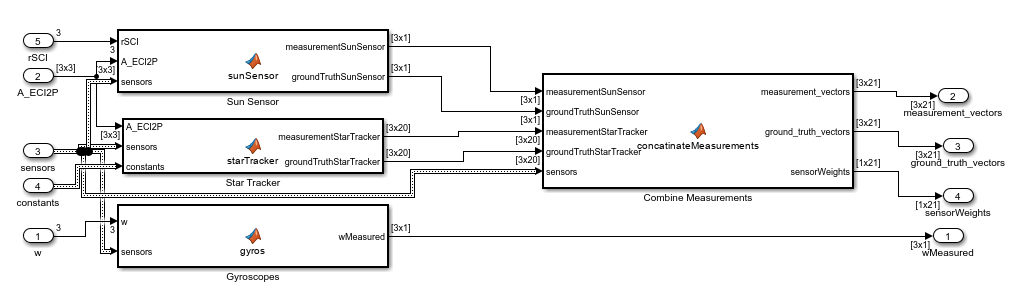
\includegraphics[scale=0.59]{Images/ps7_problem4_simulink.png}
\caption{Simulink model of sensors}
\label{fig:ps7_problem4_simulink}
\end{figure}

\begin{figure}[H]
\centering
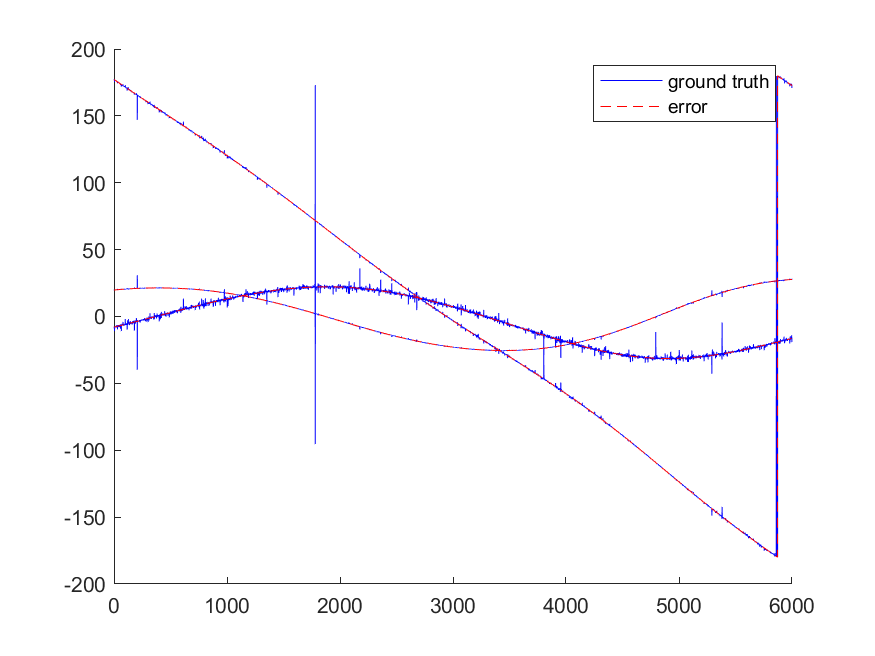
\includegraphics[scale=0.6]{Images/ps7_problem4_DADFict.png}
\caption{Attitude error using deterministic attitude determination}
\label{fig:ps7_problem4_DADFict}
\end{figure}

\begin{figure}[H]
\centering
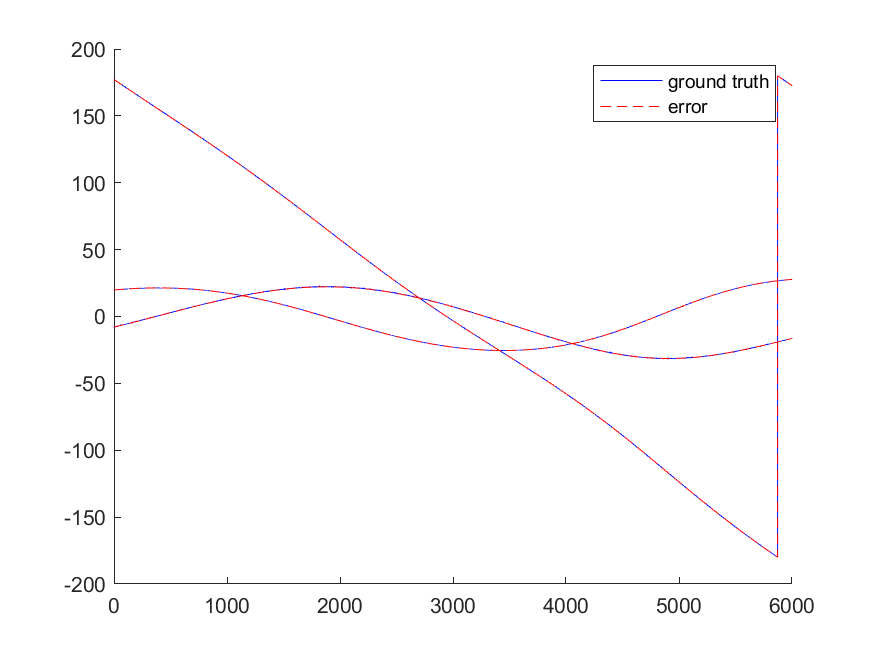
\includegraphics[scale=0.6]{Images/ps7_problem4_qMethod.png}
\caption{Attitude error using q-method}
\label{fig:ps7_problem4_qMethod}
\end{figure}

\begin{figure}[H]
\centering
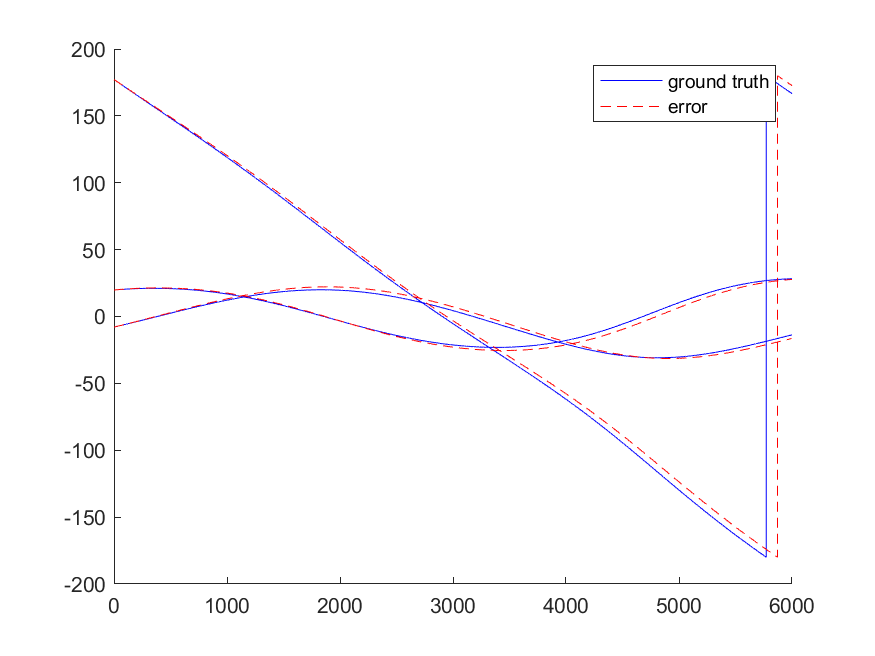
\includegraphics[scale=0.6]{Images/ps7_problem4_kin.png}
\caption{Attitude error using kinematic attitude determination}
\label{fig:ps7_problem4_kin}
\end{figure}

\subsection{Multiplicative Extended Kalman Filter, Time Update}
The following MATLAB function is our time update-only implementation of a multiplicative extended Kalman filter (MEKF). We describe the formulation of the MEKF immediately following this function.

\lstinputlisting{src/timeUpdate.m}

Our state consists of 3 small angles (zero mean) and angular velocities. Our state does not track the attitude directly, but we can compute quaternions using known kinematics.
\begin{align*}
    \Vec{x} = \begin{bmatrix}
        \alpha_{x} & \alpha_{y} & \alpha_{z} & \omega_{x} & \omega_{y} & \omega{z}
    \end{bmatrix}^{\intercal}
\end{align*}
The small angle component of our state is reset every iteration and not updated in the time update step \cite{CubeSatTelescope}.
\begin{align*}
    A &= I_{3} + \frac{s_{\omega}}{\omega} [\Vec{\omega}_{t} \times] + \frac{1 - c_{\omega}}{\omega^{2}} [\Vec{\omega}_{t} \times] [\Vec{\omega}_{t} \times] \\
    \Phi_{\omega} & = I_{3} + \Delta t \begin{bmatrix}
        0 & \frac{I_{y} - I_{z}}{I_x} \omega_{z_{t}} & \frac{I_{y} - I_{z}}{I_x} \omega_{y_{t}} \\
        \frac{I_{z} - I_{x}}{I_y} \omega_{z_{t}} & 0 & \frac{I_{z} - I_{x}}{I_y} \omega_{x_{t}} \\
        \frac{I_{x} - I_{y}}{I_z} \omega_{y_{t}} & \frac{I_{x} - I_{y}}{I_z} \omega_{x_{t}} & 0
    \end{bmatrix} \\
    \Phi &= \begin{bmatrix}
        A & 0 \\
        0 & \Phi_{\omega}
    \end{bmatrix}
\end{align*}
Since we are using a MEKF, we propagate the quaternion attitude representation outside of the state vector. The quaternion attitude is propagated by $\Omega (\Vec{\omega})$, identical to the quaternion kinematics used previously.

We plot the attitude from our MEKF and our numerical integration simulation, respectively. Upon inspection, these plots appear identical. Small errors in the simulation are analyzed later.

\begin{figure}[H]
\centering
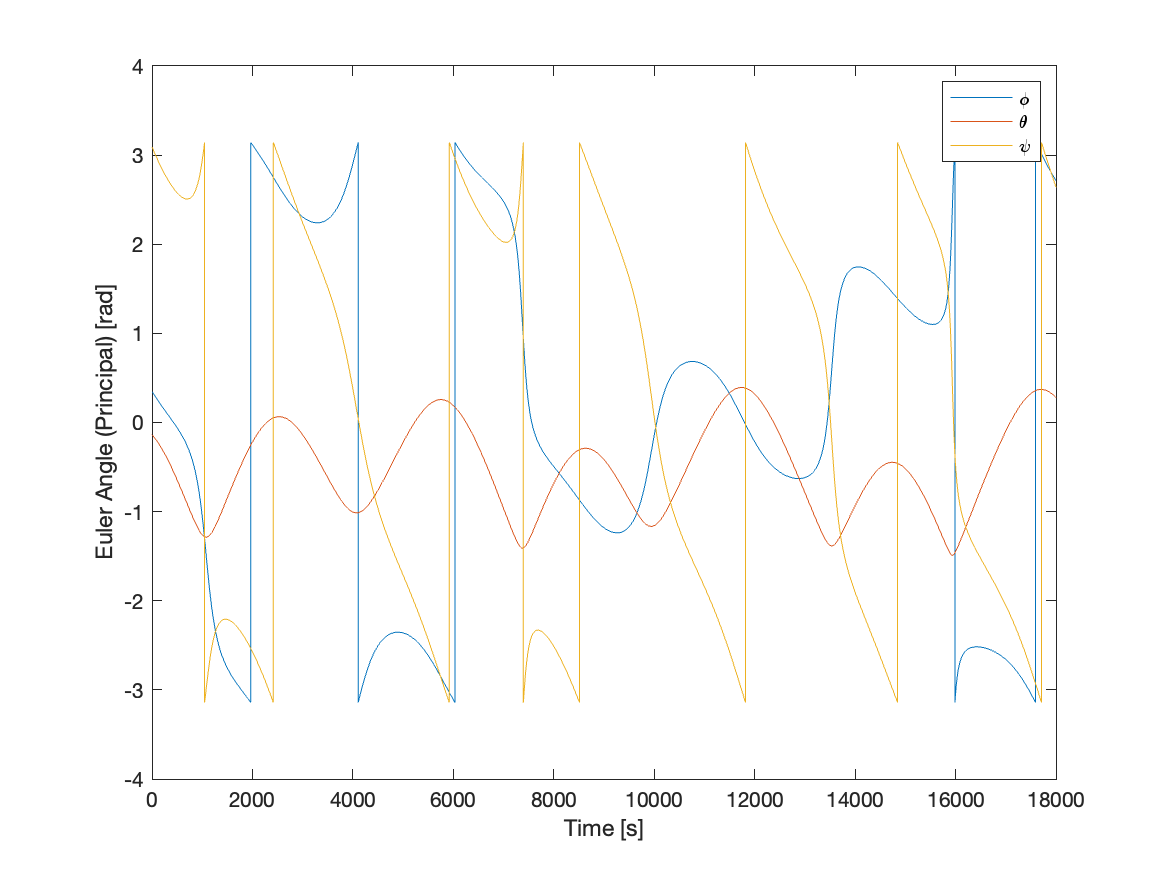
\includegraphics[scale=0.6]{Images/ps7_problem5a_angle_est.png}
\caption{Attitude evolution based on MEKF time update}
\label{fig:ps7_problem5a_angle_est}
\end{figure}

\begin{figure}[H]
\centering
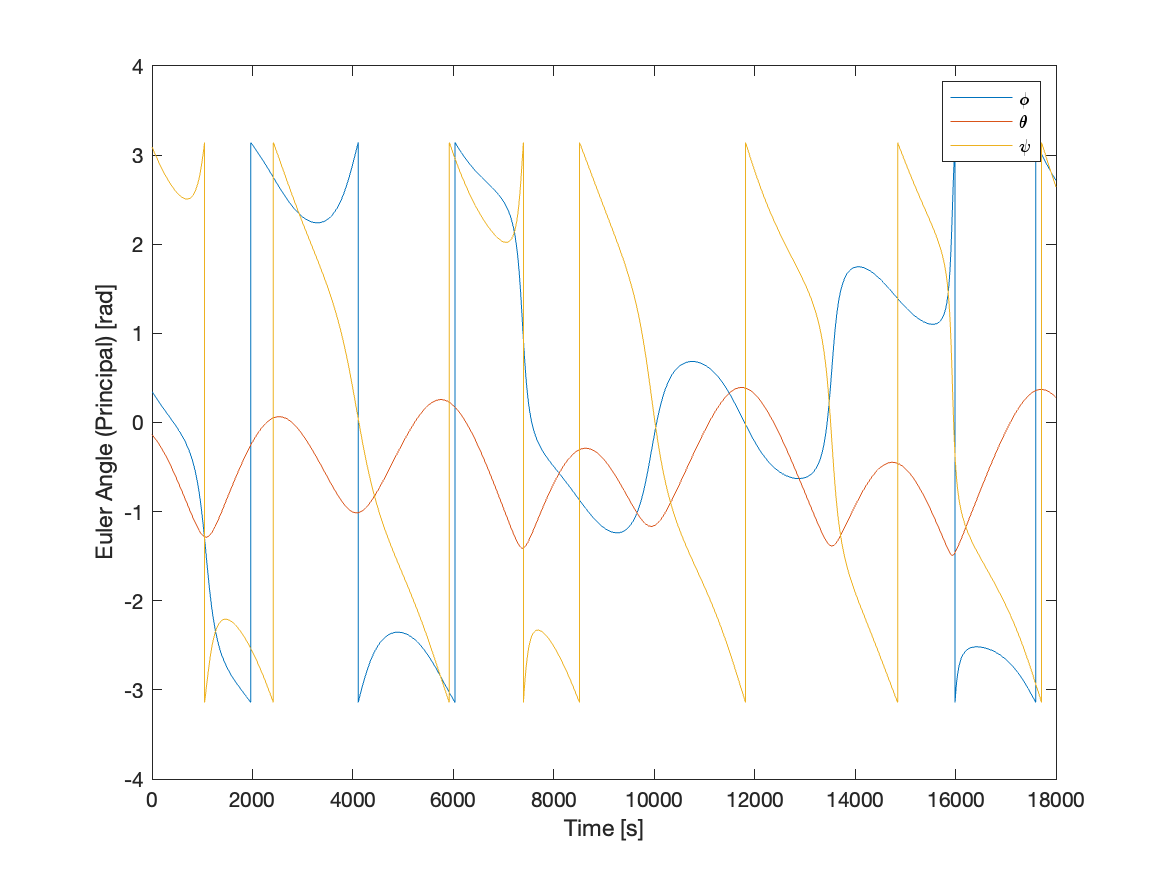
\includegraphics[scale=0.6]{Images/ps7_problem5a_angle_sim.png}
\caption{Attitude evolution from "ground truth" simulation}
\label{fig:ps7_problem5a_angle_sim}
\end{figure}

We also plot the angular velocity from both the MEKF time update step and the numerical simulation. As with the attitude evolution, both plots appear to be the same. Note that we do not include perturbations in our simulation in our comparison, as the state would quickly diverge otherwise because the measurement update is not yet implemented in the MEKF.

\begin{figure}[H]
\centering
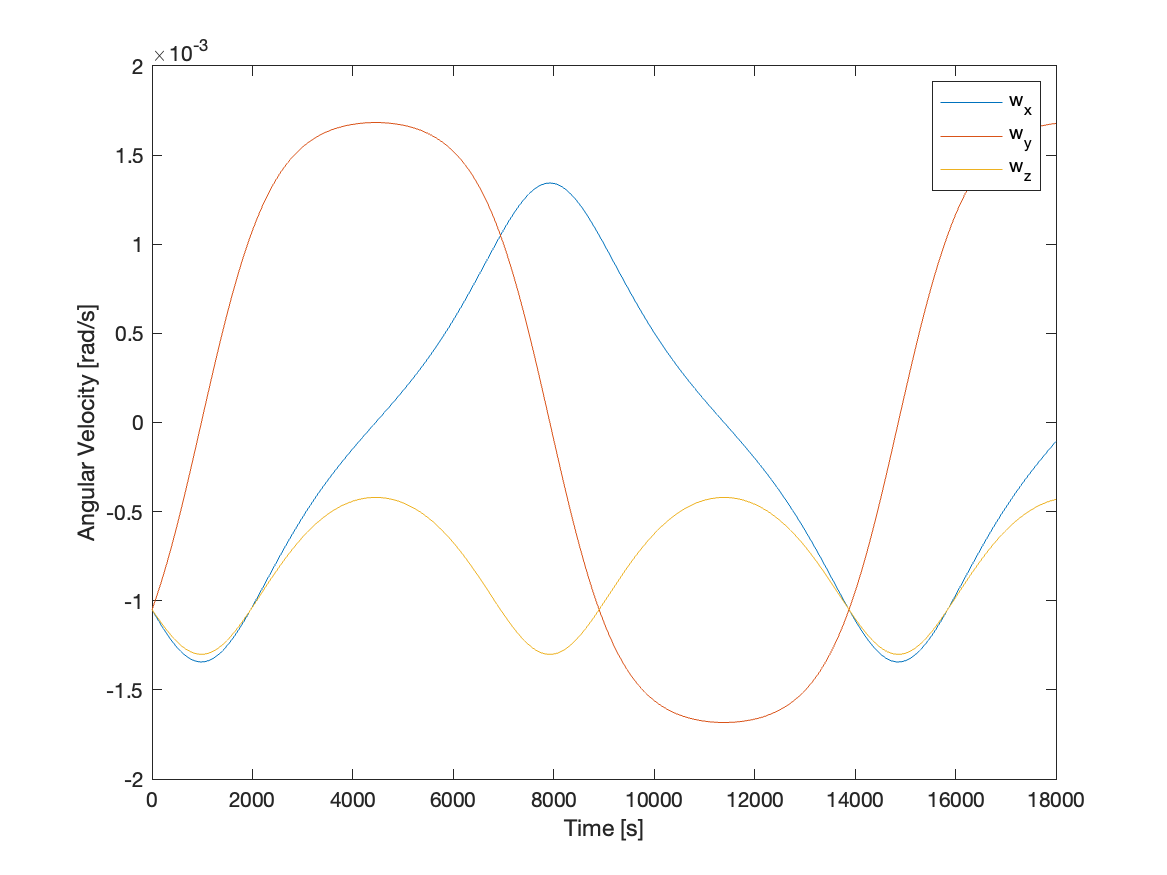
\includegraphics[scale=0.6]{Images/ps7_problem5a_angvel_est.png}
\caption{Angular velocity based on MEKF time update}
\label{fig:ps7_problem5a_angvel_est}
\end{figure}

\begin{figure}[H]
\centering
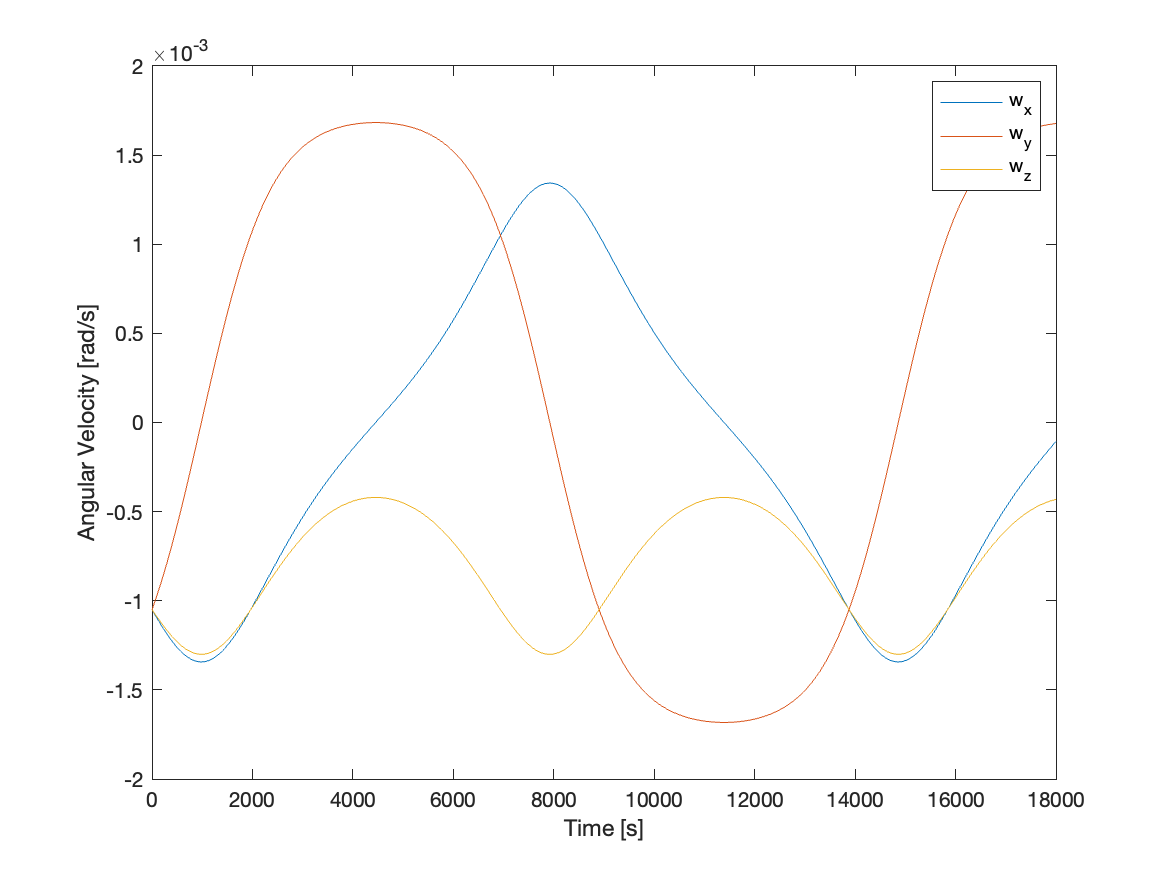
\includegraphics[scale=0.6]{Images/ps7_problem5a_angvel_sim.png}
\caption{Angular velocity from "ground truth" simulation}
\label{fig:ps7_problem5a_angvel_sim}
\end{figure}

For now, we choose to model our control inputs as torque inputs (moments) about the principal axes. Thus, we can choose a $B$ matrix as follows:
\begin{align*}
    u_{t} &= \begin{bmatrix}
        M_{x_{t}} & M_{y_{t}} & M_{z_{t}}
    \end{bmatrix} \\
    B &= \Delta t \begin{bmatrix}
        \frac{1}{I_{x}} & 0 & 0 \\
        0 & \frac{1}{I_{y}} & 0 \\
        0 & 0 & \frac{1}{I_{z}}
    \end{bmatrix}
\end{align*}
We have not yet implemented a controller at this step. As such, we will run the MEKF with $u_{t} = 0$ for now.

We can choose our initial state error covariance matrix $P$ as a diagonal matrix, with the diagonal entries corresponding to $\alpha$ set to $1$ and the entries corresponding to $\omega$ to the variance computed from angular velocity history. This can be collected as statistics from the propagation shown previously. Once the entire MEKF is implemented, this matrix should converge over time. For now, the state error covariance matrix $P$ has no impact on the output of just our time update.

For the purpose of this section, we arbitrarily define $Q = P_{t=0} \times 0.01$.

For just the time update, we show plots of errors for the attitude and angular velocity. We can see that the angular velocity error is very low, reaching a maximum of $10^{-7}$ over three orbits. Note that our raw attitude representation is in quaternions, but we convert to Euler angles for visualization. The Euler angle error is somewhat larger, beginning initially around $10^{-7}$ and ending around $10^{-3}$ over the course of the three orbits. The Euler angle error is possibly larger because there is a compounding effect of errors in computing angular velocity.

\begin{figure}[H]
\centering
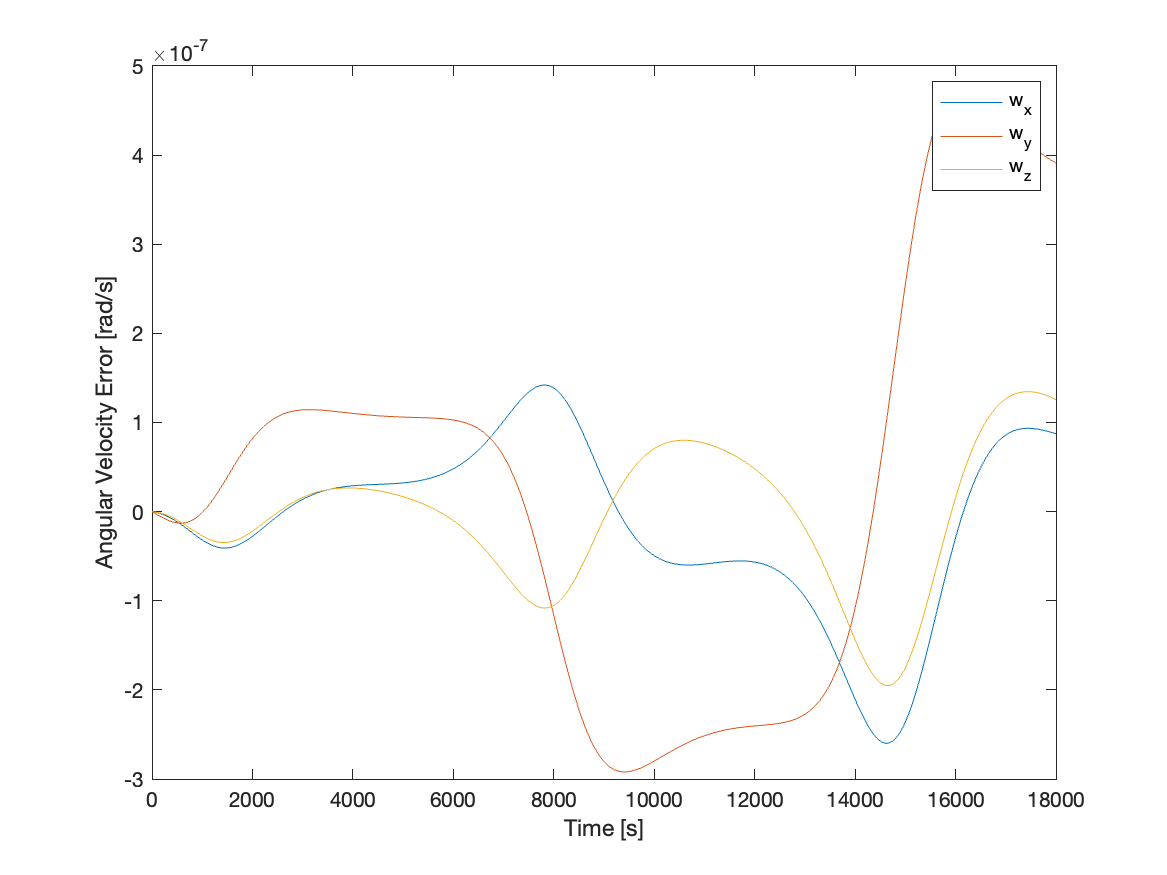
\includegraphics[scale=0.6]{Images/ps7_problem6_angvel_err.png}
\caption{Attitude error between estimate and simulation}
\label{fig:ps7_problem6_angvel_err}
\end{figure}

\begin{figure}[H]
\centering
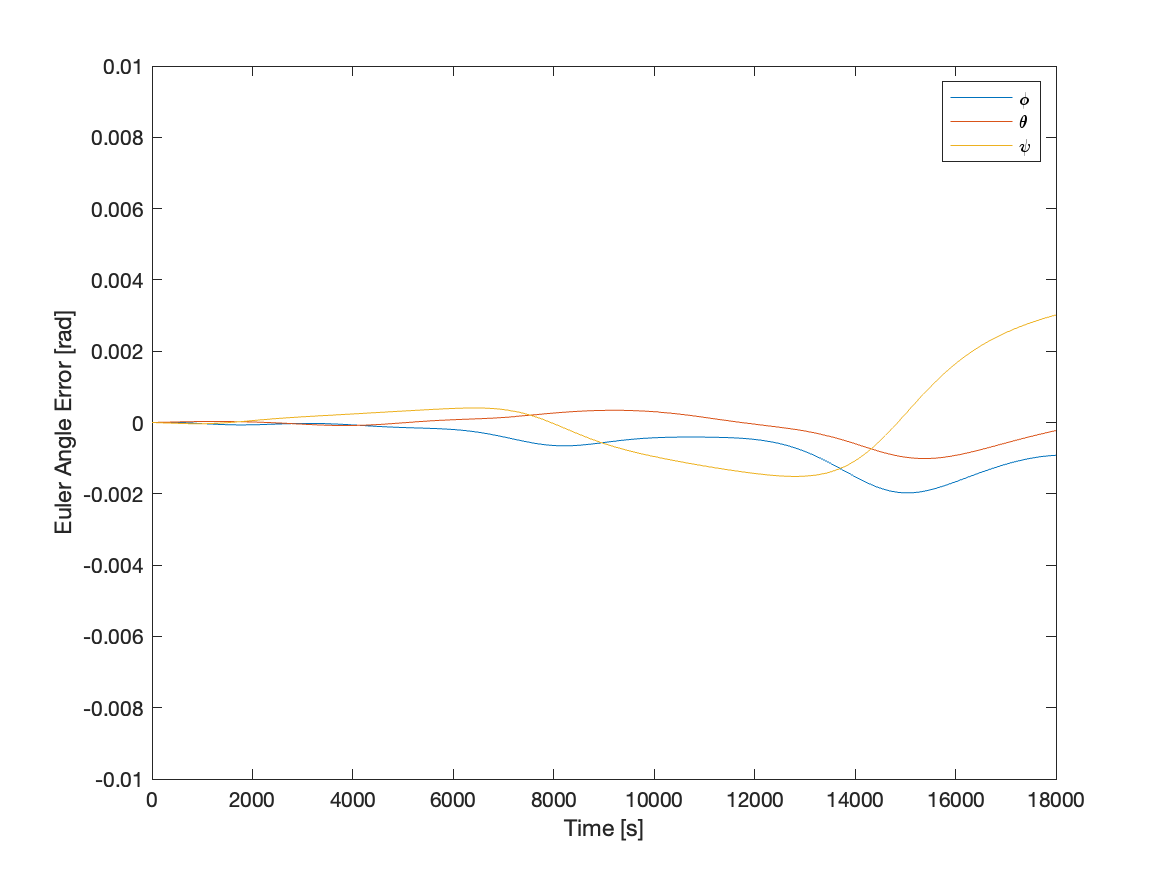
\includegraphics[scale=0.6]{Images/ps7_problem6_angle_err.png}
\caption{Angular velocity error between estimate and simulation}
\label{fig:ps7_problem6_angle_err}
\end{figure}

These results are within expectations, as we do not have a modeled measurement update step that could help reduce our errors. Also, our injected process noise $Q$ is not beneficial to the time update alone, as $Q$ is intended to help accommodate measurement updates.

\subsection{Multiplicative Extended Kalman Filter, Measurement Update}
For our measurement, we require a sensitivity matrix. The following equations define the sensitivity matrix $\mathbf{H_k}$ for the case where there are $n$ unit direction vector measurements (sun sensors, star trackers, etc.), and a 3-axis rate gyroscope measurement.
\begin{align*}
    \mathbf{H} = \frac{\delta \mathbf{h}}{\delta \mathbf{x}} =
    \begin{bmatrix}
        [\mathbf{h_1} \times] & \mathbf{0}_{3 \times 3} \\
        [\mathbf{h_2} \times] & \mathbf{0}_{3 \times 3} \\
        ... & ... \\
        [\mathbf{h_n} \times] & \mathbf{0}_{3 \times 3} \\
        \mathbf{0}_{3 \times 3} & \mathbf{I}_{3 \times 3} \\
    \end{bmatrix}
\end{align*}
In the equation above, $[\mathbf{h_i} \times]$ refers to the cross-product matrix for the measurement vector $\mathbf{h_i}$.

For the sensors used in our measurements, $\mathbf{R}$ is defined as a diagonal matrix of the sensor variances discussed in Problem Set 7, Problem 1 (where the sensor errors are based on the variance of the white noise in each case).
\begin{align*}
    \mathbf{R} = 
    \begin{bmatrix}
        diag(\sigma_{star tracker}^2) & \mathbf{0} & \mathbf{0} \\
        \mathbf{0} & diag(\sigma_{sun sensor}^2) & \mathbf{0} \\
        \mathbf{0} & \mathbf{0} & diag(\sigma_{gyroscopes}^2)\\
    \end{bmatrix}
\end{align*}
The modeled measurement vector at step k+1 was found by plugging the estimated state at step k+1 into the previously developed measurement model, without measurement noise.

Our modeled measurement uses simulated unit vectors describing directions for a star tracker and sun sensor. We also provide angular velocity data from simulation with noise to simulate a rate gyro. Our functions for the star tracker and sun sensor in the modeled measurements are shown in the appendix.

The pre-fit residuals were calculated as the difference of the output (raw measurements with noise) and the modeled measurements based on our the measurement model and state prior to the measurement update.

The following equations are used in the measurement step calculation.
\begin{align*}
    \mathbf{x_{k+1 | k+1}} = \mathbf{x_{k+1 | k}} + \mathbf{K_k}
    (\mathbf{y_k} - \mathbf{z_k}) \\
    \mathbf{P_{k+1 | k+1}} = \mathbf{P_{k+1 | k}} - 
    \mathbf{K_k} \mathbf{H_k} \mathbf{P_{k+1 | k}} \\
    \mathbf{K_k} = \mathbf{P_{k+1 | k}} \mathbf{H_k}^T [\mathbf{H_k} \mathbf{P_{k+1 | k}} \mathbf{H_k}^T + \mathbf{R_k}]^{-1}
\end{align*}
We implement the measurement update in code with the following function. This MATLAB function is used as part of our Simulink model.

\lstinputlisting{src/measurementUpdate.m}

Our entire MEKF is modeled in Simulink, as shown in the diagram below.

\begin{figure}[H]
\centering
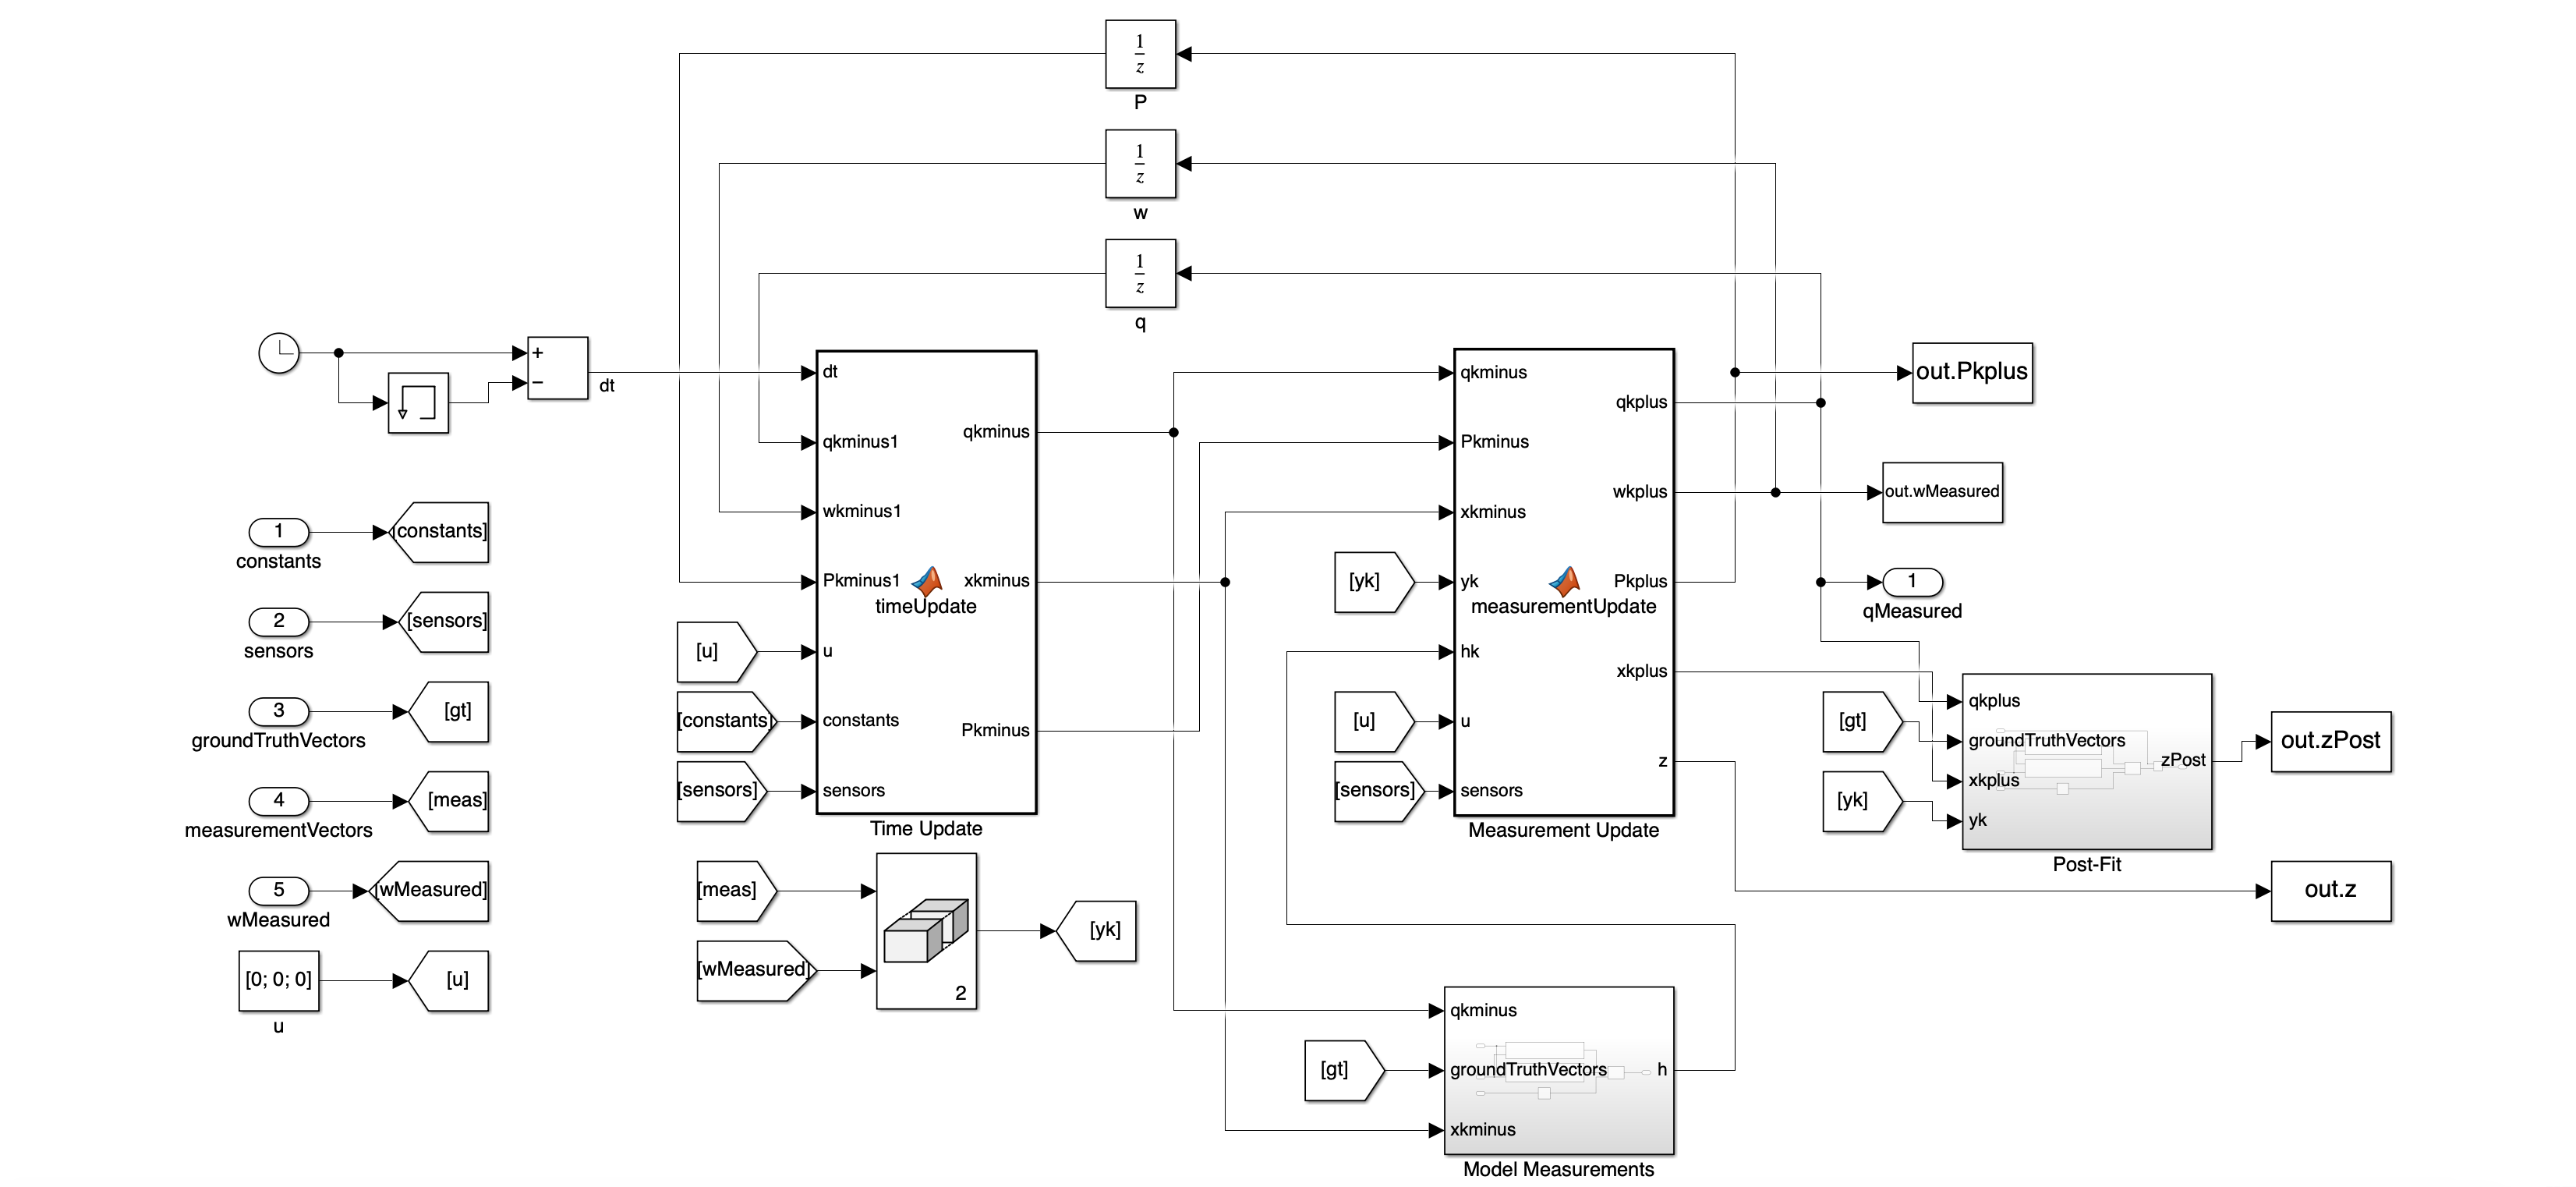
\includegraphics[scale=0.27]{Images/ps8_problem5_simulink.png}
\caption{Simulink model of MEKF}
\label{fig:ps8_problem5_simulink}
\end{figure}

\subsection{Multiplicative Extended Kalman Filter, Errors}
Figure \ref{fig:ps8_problem7_error} shows the attitude estimate errors with the MEKF method. As expected, the errors are very small compared to the attitude determination methods used in the previous section.

Figure \ref{fig:ps8_problem7_cov} shows the estimated attitude determination errors based on the covariance of the filter. Comparing this with Figure \ref{fig:ps8_problem7_error}, it seems that this method may under-report the error and is not necessarily the most accurate representation of error. Figure \ref{fig:ps8_problem7_covComp}, makes the difference between these two values even clearer. In short, there is are multiple orders of magnitude difference between the actual error and what the covariance bounds would predict. This could be caused by a couple of factors. After further inspection, it seems that the small covariance values come from the measurement step, where they get shrunken from roughly $1-2 \deg$ to the tiny values plotted. It seems possible that the values in the \textbf{R} matrix might be too low, suggesting that the measurement are being trusted too much, leading to covaraince values that are too low. Tuning the \textbf{R} matrix more could lower this value; however, the current estimate has proven effective in state estimation.

\begin{figure}[H]
\centering
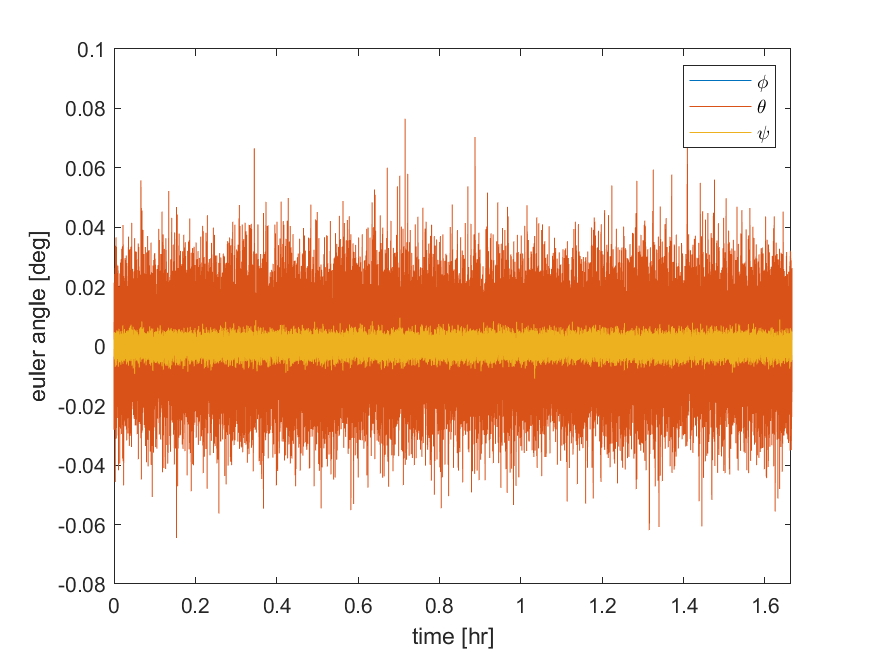
\includegraphics[scale=0.8]{Images/ps8_problem7_error.png}
\caption{Errors between MEKF measurements and ground truth}
\label{fig:ps8_problem7_error}
\end{figure}

\begin{figure}[H]
\centering
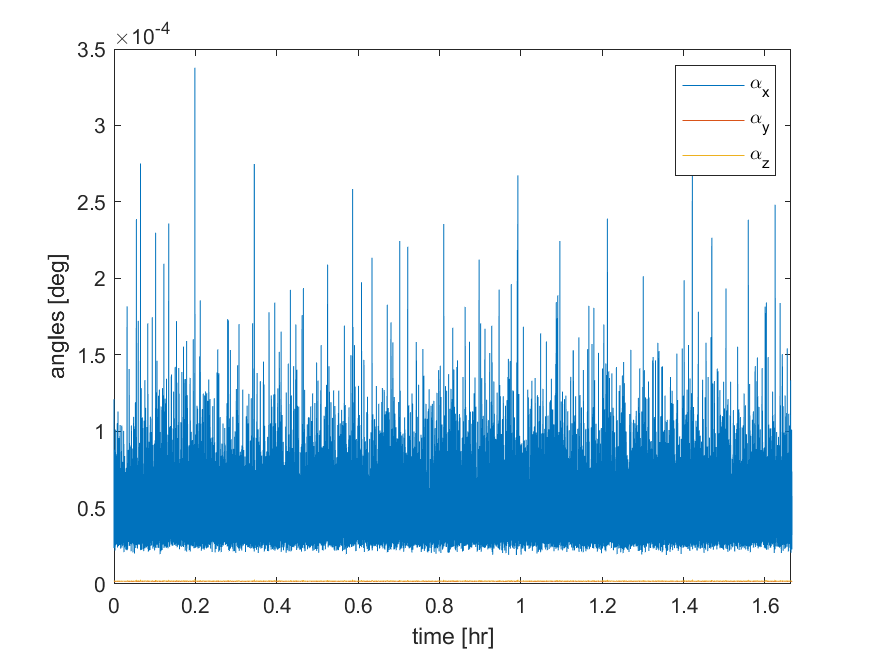
\includegraphics[scale=0.8]{Images/ps8_problem7_cov.png}
\caption{Estimated attitude estimation errors from covariance (small angles)}
\label{fig:ps8_problem7_cov}
\end{figure}

\begin{figure}[H]
\centering
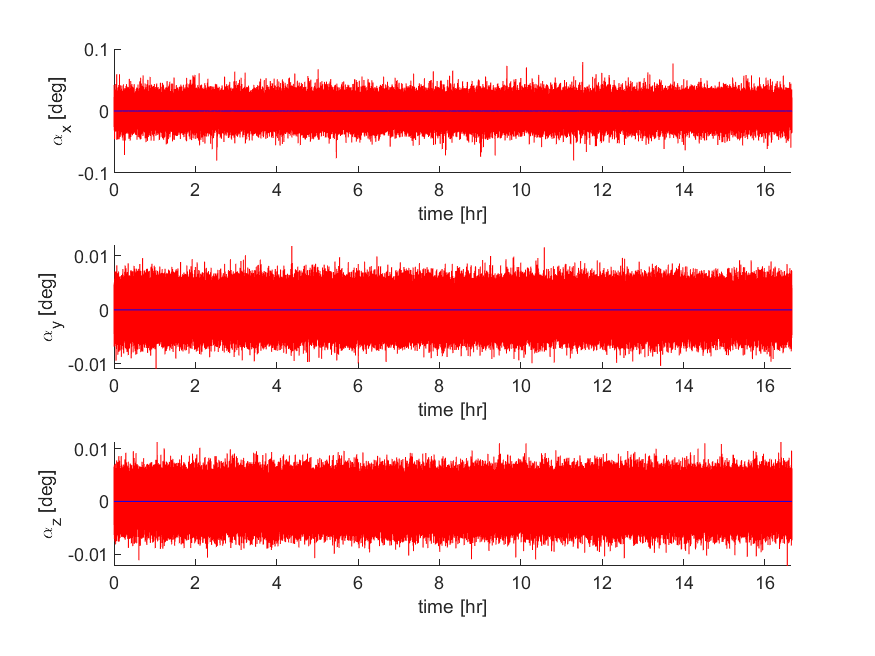
\includegraphics[scale=0.8]{Images/ps8_problem7_covComp.png}
\caption{Estimated Error (95\% confidence interval) vs Actual Errors}
\label{fig:ps8_problem7_covComp}
\end{figure}

The post-fit residuals z are found by taking the updated state from the measurement update step and computing a modeled measurement using our measurement model again. Figures \ref{fig:ps8_problem7_res_units} and \ref{fig:ps8_problem7_res_gyro} below show the difference in the norms of the pre-fit and post-fit residuals. As expected, the post-fit residuals are slightly smaller than the pre-fit residuals. However, the difference between pre-fit and post-fit sensor noise is much better for the gyroscope measurements than the unit direction vector measurements.

\begin{figure}[H]
\centering
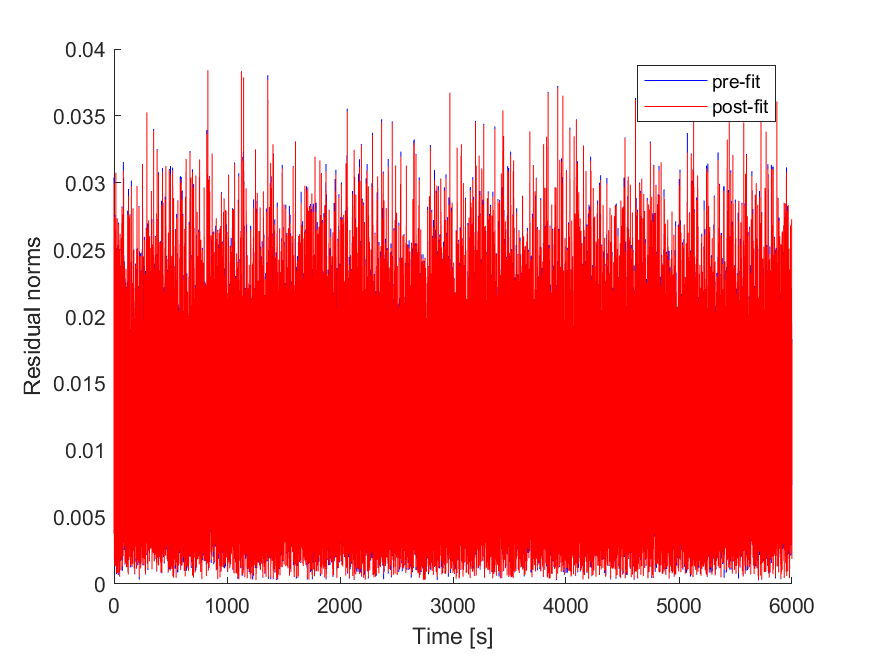
\includegraphics[scale=0.8]{Images/ps8_problem7_res_units.png}
\caption{Norm of pre-fit and post-fit direction-vector residuals}
\label{fig:ps8_problem7_res_units}
\end{figure}

\begin{figure}[H]
\centering
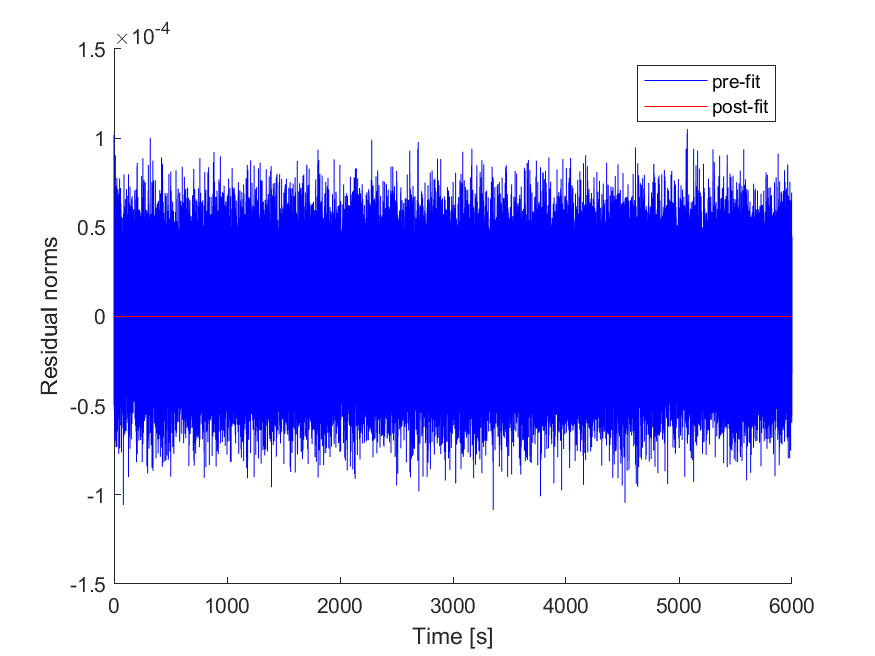
\includegraphics[scale=0.8]{Images/ps8_problem7_res_gyro.png}
\caption{Pre-fit and post-fit gyroscope residuals}
\label{fig:ps8_problem7_res_gyro}
\end{figure}

Investigating the measurement model, noise model, and sensitivity matrix for the unit vector-based measurements, we may be able to improve the performance shown in Figure \ref{fig:ps8_problem7_res_units}. This is an area for potential future work, as well as the topics discussed in the following section.